\documentclass[a4paper]{article}

% Basic packages
\usepackage{fontspec}
\XeTeXlinebreaklocale "zh"    % 启用中文断行（XeTeX 内建，无需 xeCJK）
\XeTeXlinebreakskip = 0pt plus 1pt
\setmainfont{Songti SC}
\setsansfont{Heiti SC}
\setmonofont{Menlo}
\usepackage{amsmath, amssymb}
\usepackage{graphicx}
\usepackage[margin=2.5cm]{geometry}
\usepackage[most]{tcolorbox}
\usepackage{etoolbox}
\usepackage{listings}
\usepackage{hyperref}
\usepackage{booktabs}
\usepackage{subcaption}
\usepackage{float}

% Chinese font setup (macOS system fonts, no ctex needed)
\setmainfont{Songti SC}
\setsansfont{Heiti SC}
\setmonofont{Menlo}
\newcommand{\song}{\fontspec{Songti SC}}
\newcommand{\hei}{\fontspec{Heiti SC}}
\newcommand{\kai}{\fontspec{KaiTi}}
\newcommand{\fangsong}{\fontspec{FangSong}}

% ===== Highlight boxes =====
\newtcolorbox{knowledgebox}[1]{
    enhanced, colback=blue!5!white, colframe=blue!75!black, colbacktitle=blue!75!black,
    coltitle=white, fonttitle=\bfseries, title=#1, attach boxed title to top left={yshift=-2mm, xshift=2mm},
    boxrule=1pt, sharp corners
}

\newtcolorbox{importantbox}[1]{
    enhanced, colback=yellow!10!white, colframe=yellow!80!black, colbacktitle=yellow!80!black,
    coltitle=black, fonttitle=\bfseries, title=#1, sharp corners
}

\newtcolorbox{warningbox}[1]{
    enhanced, colback=red!5!white, colframe=red!75!black, colbacktitle=red!75!black,
    coltitle=white, fonttitle=\bfseries, title=#1, sharp corners
}

\newtcolorbox{practicebox}[1]{
    enhanced, colback=green!5!white, colframe=green!60!black, colbacktitle=green!60!black,
    coltitle=white, fonttitle=\bfseries, title=#1, sharp corners
}

% ===== Code listings =====
\lstset{
    basicstyle=\ttfamily\small,
    keywordstyle=\color{blue},
    stringstyle=\color{red!60!black},
    commentstyle=\color{green!60!black},
    breaklines=true,
    frame=single,
    numbers=left,
    numberstyle=\tiny\color{gray},
    captionpos=b,
    extendedchars=false
}

% ===== Front-page metadata =====
\newcommand{\notetitle}{CS336 Lecture 2：PyTorch 与资源核算}
\newcommand{\notesubtitle}{Stanford CS336: Language Modeling from Scratch (Spring 2025)}
\newcommand{\noteauthors}{讲师：Percy Liang \quad 笔记：ZCode}
\newcommand{\notedate}{2026-07-14}
\newcommand{\videochannel}{Stanford CS336}
\newcommand{\videopublishdate}{2025 Spring}
\newcommand{\videoduration}{79 分钟}
\newcommand{\videourl}{https://www.youtube.com/watch?v=msHyYioAyNE}
\newcommand{\videocoverpath}{cover.jpg}

\begin{document}

% ===== Title page =====
\begin{titlepage}
\centering
{\Large 课程笔记\par}
\vspace{1.2cm}
{\huge\bfseries \notetitle\par}
\vspace{0.3cm}
{\large \notesubtitle\par}
\vspace{0.5cm}
{\large \noteauthors\par}
\vspace{0.3cm}
{\large \notedate\par}
\vspace{1.0cm}

\includegraphics[width=0.82\textwidth,height=0.40\textheight,keepaspectratio]{\videocoverpath}\par

\vfill
\begin{tcolorbox}[width=0.9\textwidth, colback=black!2!white, colframe=black!60, sharp corners]
\textbf{视频作者/频道}：\videochannel\par
\textbf{发布日期}：\videopublishdate\par
\textbf{视频时长}：\videoduration\par
\textbf{视频链接}：\href{\videourl}{\nolinkurl{\videourl}}
\end{tcolorbox}
\end{titlepage}

\tableofcontents
\newpage

%% --- 正文内容开始 ---

\section{开场：为什么需要资源核算}

\subsection{本课定位}

承接第一讲的课程导论，Percy Liang 在本讲开篇明确指出本节课的两个目标。第一，过一遍构建模型所需的 PyTorch 原语（primitives）：从 tensors（张量）出发，构建 models（模型）、optimizers（优化器）和 training loop（训练循环）。第二，并贯穿始终的核心是\textbf{效率}（efficiency）——具体来说，我们究竟如何使用资源，包括 memory（内存）与 compute（算力）。

\begin{importantbox}{本讲的知识类型}
对应第一讲的"三类知识"框架：
\begin{itemize}
\item \textbf{机制（Mechanics）}：本讲主体，理解 PyTorch 在原语层如何运作，是可传授、可迁移的。
\item \textbf{心态（Mindset）}：resource accounting（资源核算）本身就是一种心态——它不难，但你\textbf{必须去做}。
\item \textbf{直觉（Intuition）}：本讲基本不涉及，重点在机制与心态的夯实。
\end{itemize}
\end{importantbox}

Percy 特别强调，本讲\textbf{不会}详细讲 Transformer 架构（那是下一讲 Tatsu 的内容），而是用更简单的线性模型来讲清楚原语和资源核算。理解 Transformer 的途径有很多：Assignment 1 的 handout、网上的图文教程。本讲的焦点是：每一份 FLOPs 去了哪里、每一字节内存被谁占用。

\subsection{用 napkin math 回答两个问题}

\begin{figure}[H]
\centering
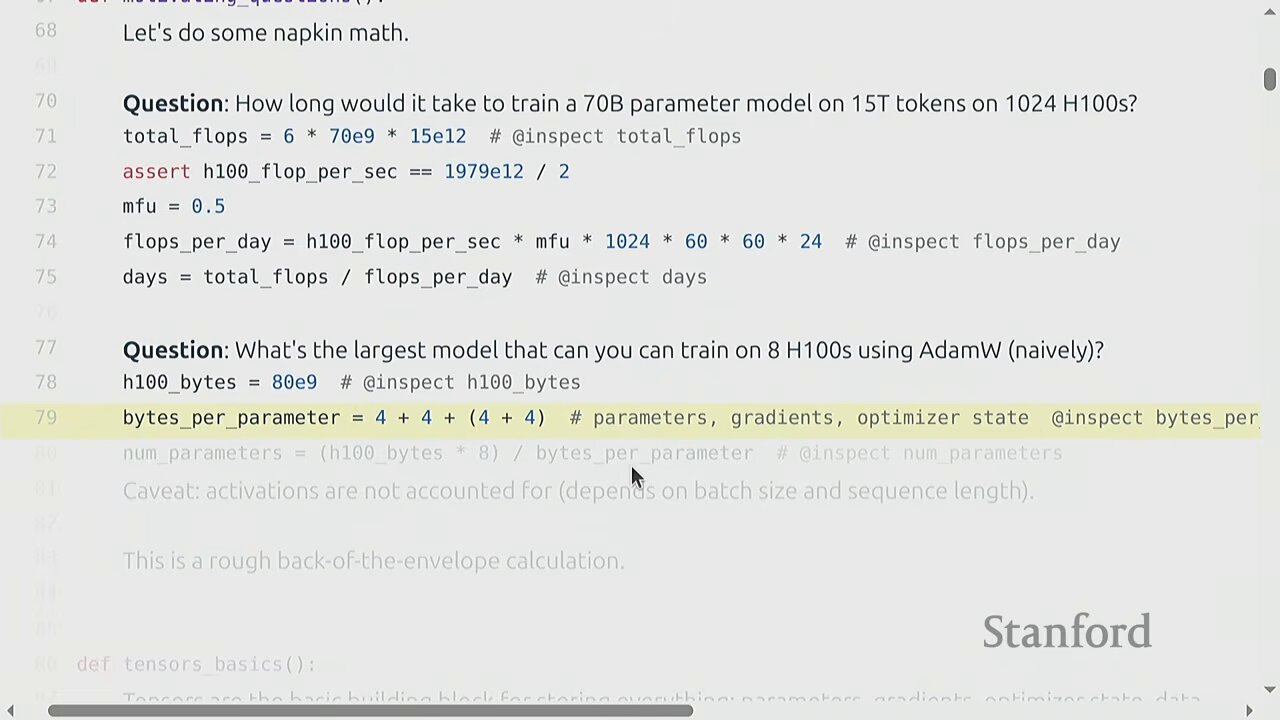
\includegraphics[width=\textwidth]{figures/fig_01_napkin_math.jpg}
\caption{开场 motivating questions：用 napkin math 估算训练成本\protect\footnotemark}
\end{figure}
\footnotetext{视频画面时间区间：02:45--03:15。}

Percy 抛出两个用"餐巾纸背面算术"（napkin math）就能回答的问题，它们正是 resource accounting 的典型应用：

\begin{importantbox}{两个 motivating questions}
\textbf{问题一}：用 1024 块 H100 训练一个 700 亿参数的 dense transformer，喂 15 万亿 token，需要多久？

\textbf{问题二}：在 8 块 H100 上用 AdamW 训练（不做太花哨的优化），能训的\textbf{最大模型}是多大？
\end{importantbox}

问题一的解答思路如下。先算训练所需的总 FLOPs：

\[
\text{FLOPs}_{\text{train}} = 6 \times N_{\text{params}} \times N_{\text{tokens}}
\]

\begin{itemize}
\item $N_{\text{params}} = 70 \times 10^9$：模型参数量
\item $N_{\text{tokens}} = 15 \times 10^{12}$：训练 token 数
\item 系数 6：每个参数在每个 token 上大约做 6 次 FLOPs（前向 2 + 反向 4，本讲后文会推导）
\end{itemize}

再算硬件每天能提供的 FLOPs。H100 的峰值算力约为 $P = 989 \times 10^{12}$ FLOPs/s（BF16），设 MFU（model FLOPs utilization）为 0.5，则 1024 块卡一天能算：

\[
\text{FLOPs}_{\text{per day}} = 1024 \times 989 \times 10^{12} \times 0.5 \times 86400
\]

两者相除即得训练天数：

\[
T_{\text{days}} = \frac{\text{FLOPs}_{\text{train}}}{\text{FLOPs}_{\text{per\_day}}} \approx 144 \text{ 天}
\]

问题二则从内存角度切入。H100 有 80GB HBM，用 AdamW 时每参数约需 16 字节（参数 4 + 梯度 4 + 优化器状态 $m, v$ 各 4，后文详述），于是：

\[
N_{\text{params}}^{\max} = \frac{8 \times 80 \times 10^9}{16} \approx 40 \times 10^9
\]

\begin{warningbox}{这是粗略估算}
这个估算\textbf{没有}算 activations（激活），而激活占用取决于 batch size 和 sequence length。本讲用线性模型回避了这点，但 Assignment 1 的 Transformer 必须把它算进去。
\end{warningbox}

\subsection{为什么要做 resource accounting}

\begin{knowledgebox}{效率是核心目标}
Percy 直言：你可能习惯了"实现一个模型、训练它、发生什么是什么"。但记住\textbf{效率是这场游戏的名字}（efficiency is the name of the game）。要高效，你必须精确知道自己到底消耗了多少 FLOPs——因为当这些数字变大时，它们\textbf{直接换算成美元}，你希望它尽可能小。
\end{knowledgebox}

本讲的思路是：先讲 memory accounting（内存核算），再讲 compute accounting（算力核算），最后自底向上把模型搭起来。

\section{内存核算：Tensor 与浮点数}

\subsection{Tensor：深度学习的一切都存在这里}

Tensor（张量）是深度学习中存储一切的构建块（building block）：parameters（参数）、gradients（梯度）、optimizer state（优化器状态）、data（数据）、activations（激活），都是 tensor。你可以用多种方式创建 tensor，也可以创建一个未初始化的 tensor 然后用特殊初始化方法填充参数。

\begin{figure}[H]
\centering
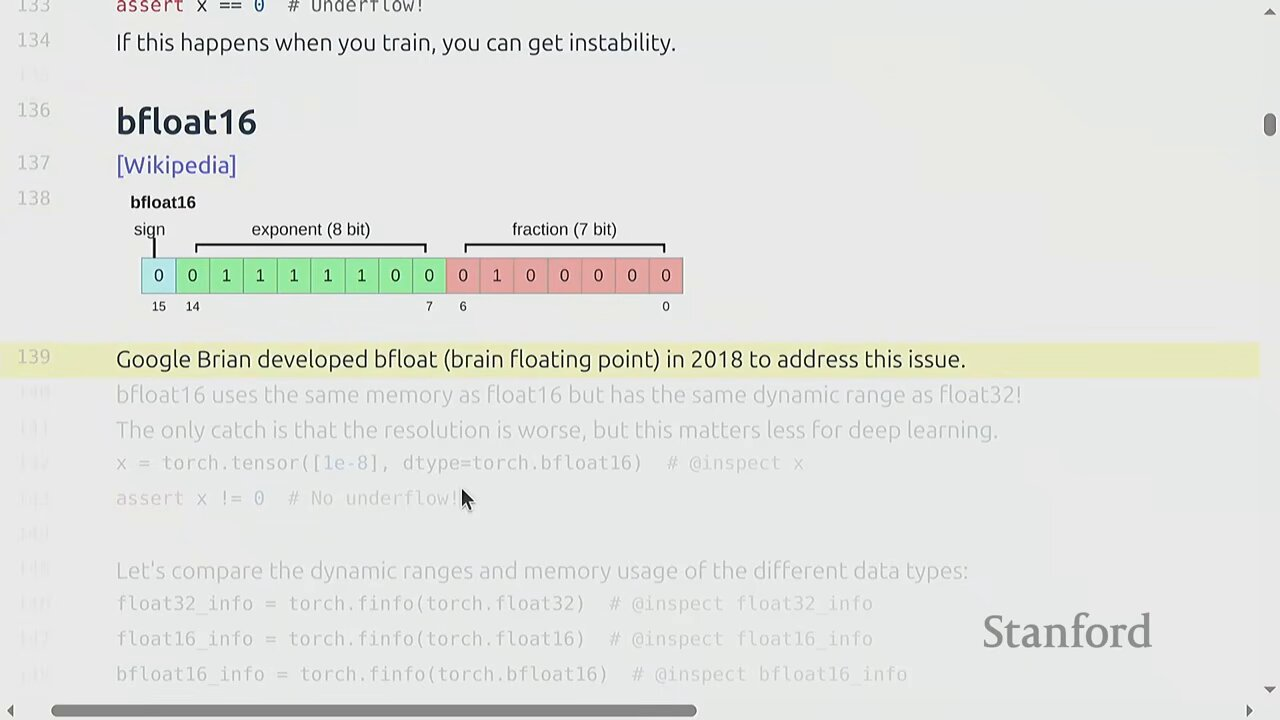
\includegraphics[width=\textwidth]{figures/fig_05_tensor_memory.jpg}
\caption{Tensor 内存计算：一个 4×8 的 float32 矩阵占 128 字节\protect\footnotemark}
\end{figure}
\footnotetext{视频画面时间区间：10:00--10:30。}

\subsection{浮点数格式}

我们感兴趣的每个 tensor 几乎都以 floating-point number（浮点数）形式存储。浮点数有多种表示方式，理解它们的位结构是内存核算的基础。

\begin{figure}[H]
\centering
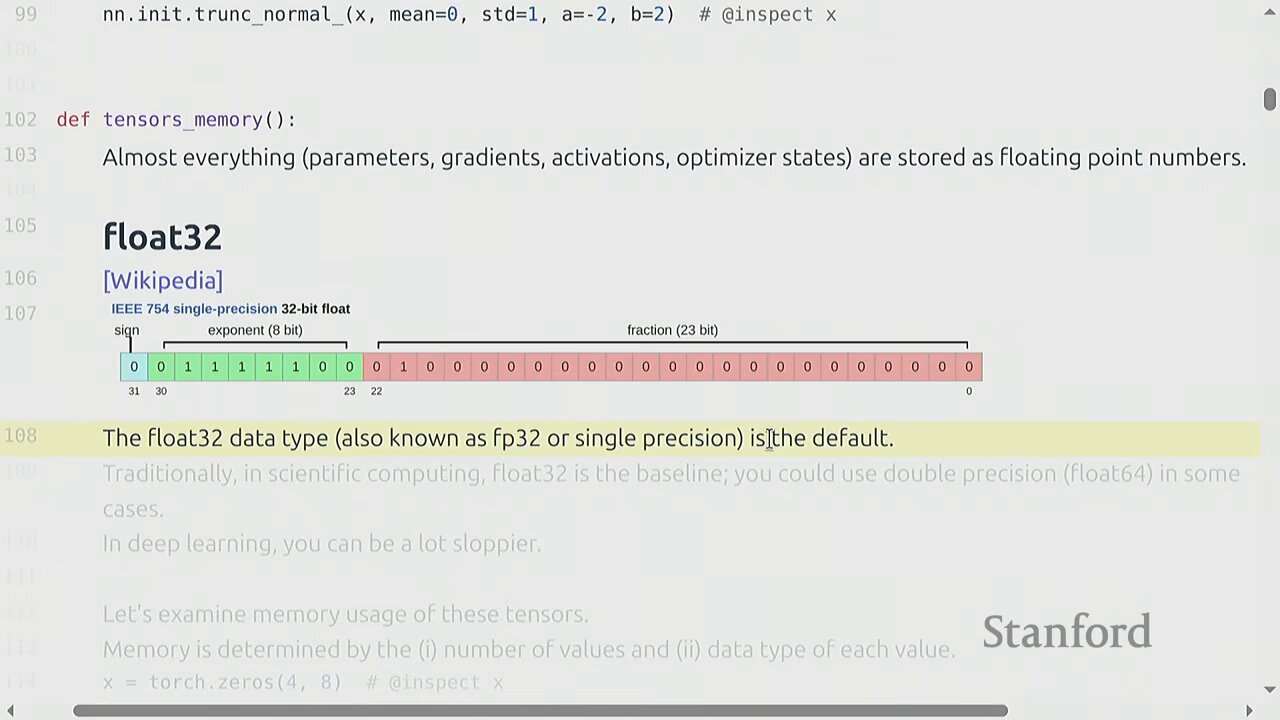
\includegraphics[width=\textwidth]{figures/fig_02_fp32_bits.jpg}
\caption{FP32（单精度）位结构：1 sign + 8 exponent + 23 fraction = 32 bits\protect\footnotemark}
\end{figure}
\footnotetext{视频画面时间区间：06:45--07:15。}

\subsubsection{FP32（float32 / single precision）}

最默认的方式是 float32（FP32），共 32 位：1 位 sign（符号）、8 位 exponent（指数）、23 位 fraction（尾数/小数部分）。Exponent 决定 dynamic range（动态范围），fraction 决定能表示多少不同的值。FP32 也叫 single precision（单精度），是计算的"黄金标准"，机器学习里常称为 full precision（全精度）。

\begin{knowledgebox}{"full precision"是相对的}
科学计算的人听到 FP32 叫"全精度"会笑——他们用 float64 甚至更高。但对机器学习而言，FP32 几乎是你需要的上限，因为深度学习本身就是"sloppy"（粗放）的。
\end{knowledgebox}

\subsubsection{FP16 vs BF16}

\begin{figure}[H]
\centering
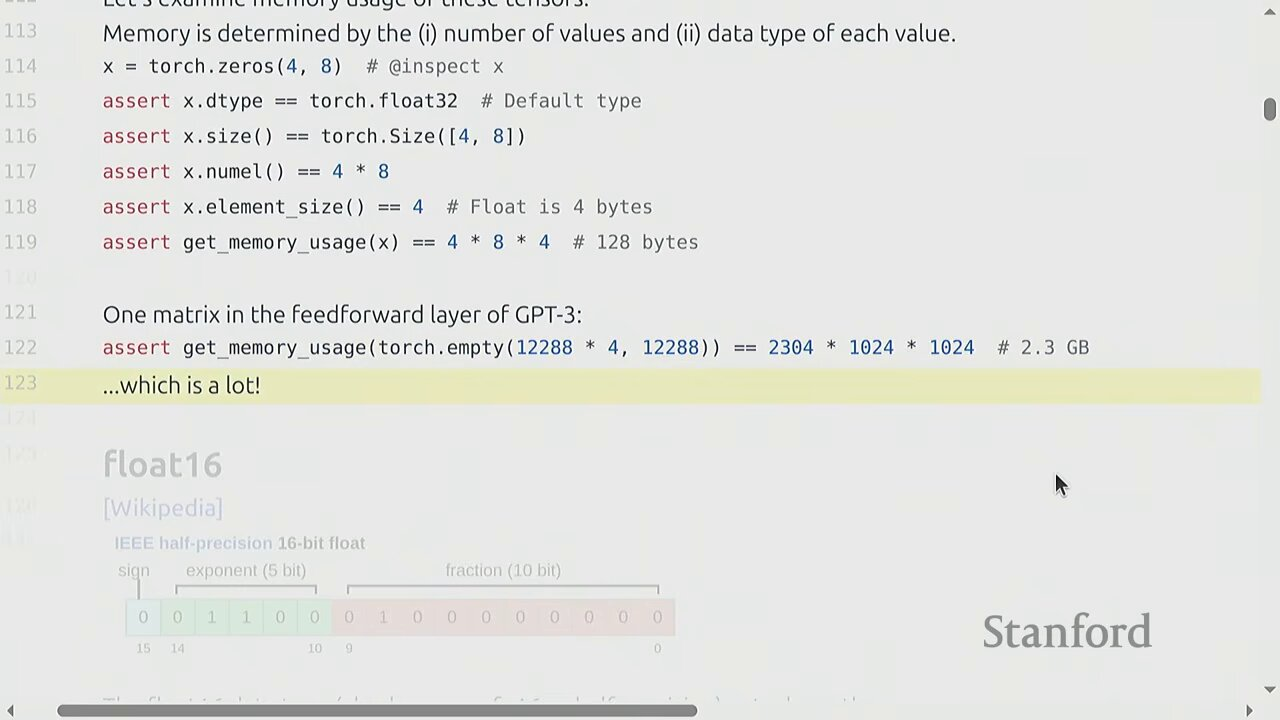
\includegraphics[width=\textwidth]{figures/fig_03_fp16_bf16_compare.jpg}
\caption{FP16 vs BF16 对比：FP16(1+5+10) 动态范围小易溢出，BF16(1+8+7) 与 FP32 同动态范围\protect\footnotemark}
\end{figure}
\footnotetext{视频画面时间区间：08:15--08:45。}

除了 FP32，还有两种 16 位格式。FP16 把 exponent 从 8 缩到 5、fraction 从 23 缩到 10。但 FP16 的\textbf{致命问题}是动态范围太小（5 位 exponent），训练时梯度很容易 overflow（溢出）或 underflow（下溢）。

\begin{figure}[H]
\centering
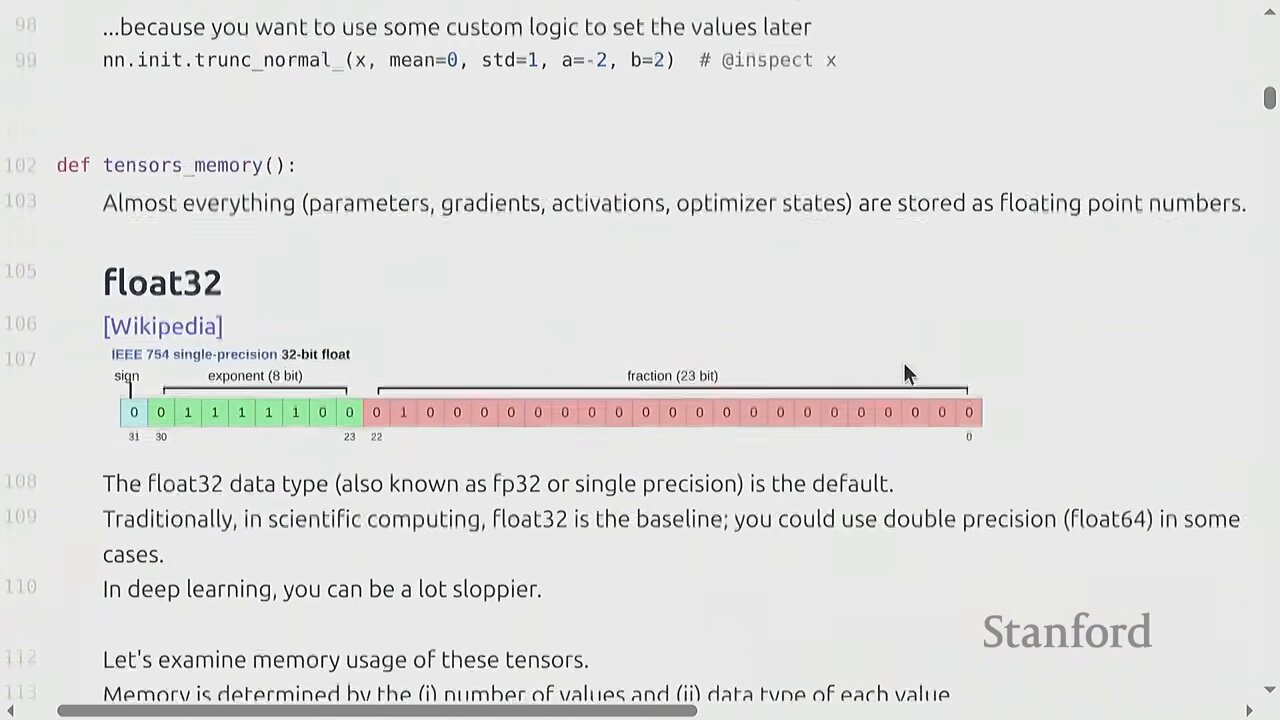
\includegraphics[width=\textwidth]{figures/fig_04_bf16_layout.jpg}
\caption{BF16（brain float）：保留 FP32 的 8 位 exponent，牺牲 fraction，专为深度学习设计\protect\footnotemark}
\end{figure}
\footnotetext{视频画面时间区间：08:45--09:15。}

\textbf{BF16}（bfloat16，brain float）是更好的选择。它的位结构是 1 sign + 8 exponent + 7 fraction——\textbf{exponent 位数与 FP32 完全相同}，因此动态范围与 FP32 一致，只是精度（fraction）更低。这意味着你可以把 FP32 数值直接截断（truncate）成 BF16 而不改变其量级，训练稳定性远好于 FP16。BF16 由 Google Brain 团队开发，因此得名"brain float"。

\begin{importantbox}{BF16 是训练的事实标准}
BF16 把 exponent（动态范围）看得比 fraction（精度）更重要，因为深度学习对动态范围更敏感、对精度更宽容。在 H100 这类现代硬件上，BF16 的峰值算力远高于 FP32。本课与工业界的训练默认都用 BF16。
\end{importantbox}

\subsection{Tensor 的内存占用}

Tensor 的内存占用非常简单，由两个量决定：

\[
\text{memory} = \text{num\_elements} \times \text{bytes\_per\_element}
\]

例如创建一个 $4 \times 8$ 的 float32 tensor：元素数 $= 32$，每个元素 4 字节，总内存 $= 128$ 字节。可以用 \texttt{tensor.element\_size()}（每个元素字节数）和 \texttt{tensor.numel()}（元素总数）来查询。

\subsubsection{混合精度训练}

\begin{figure}[H]
\centering
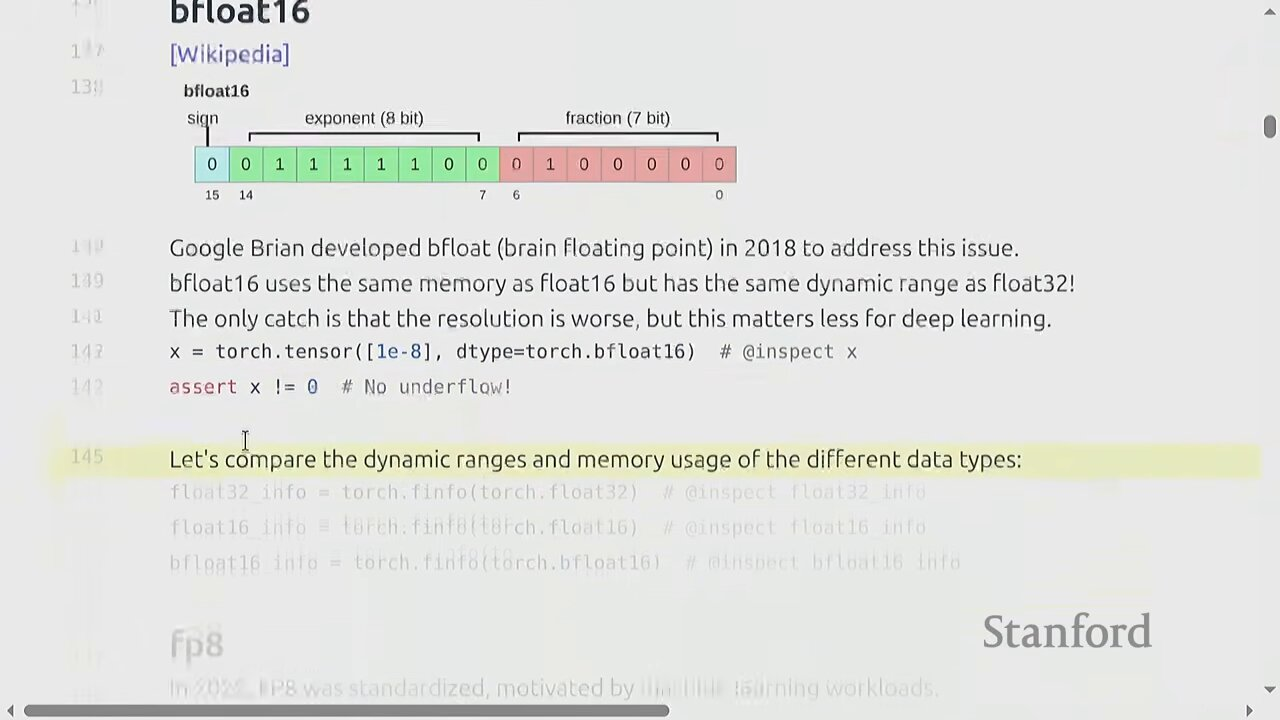
\includegraphics[width=\textwidth]{figures/fig_06_mixed_precision.jpg}
\caption{混合精度训练：BF16 做前向/反向计算，FP32 保存 master weights 做参数更新\protect\footnotemark}
\end{figure}
\footnotetext{视频画面时间区间：10:45--11:15。}

\textbf{Mixed precision training}（混合精度训练）是工程上的折中。核心思路：用低精度（BF16/FP16）做前向和反向的\textbf{计算}以节省时间和内存，但保留一份 FP32 的 \textbf{master weights}（主权重副本）用于参数更新，保证数值稳定性。这是因为梯度累加和参数更新对精度敏感，若全程用低精度会导致训练不稳定。

\begin{practicebox}{什么时候用 FP32，什么时候用 BF16}
\begin{itemize}
\item 前向/反向的大规模 matmul：用 BF16（快、省内存）
\item 参数更新、梯度累加、optimizer state：用 FP32（稳定）
\item 默认推荐：尽可能用 BF16 甚至 FP8 做前向，其余用 FP32
\end{itemize}
\end{practicebox}

\subsection{Views、Strides 与 Contiguous}

理解 tensor 在内存中如何布局，对高效代码至关重要。PyTorch 的 tensor 并不总是连续存储——它通过 \textbf{strides}（步幅）来描述如何遍历数据。底层上，任何 tensor 的实际数据都存在一段一维的连续内存里，而 tensor 的"形状"只是一个逻辑视图：它告诉 PyTorch 如何用 strides 去索引这段一维存储。掌握这套机制，你就能预测哪些操作会拷贝数据（昂贵的）、哪些不会（便宜的），从而写出内存高效的代码。

\begin{figure}[H]
\centering
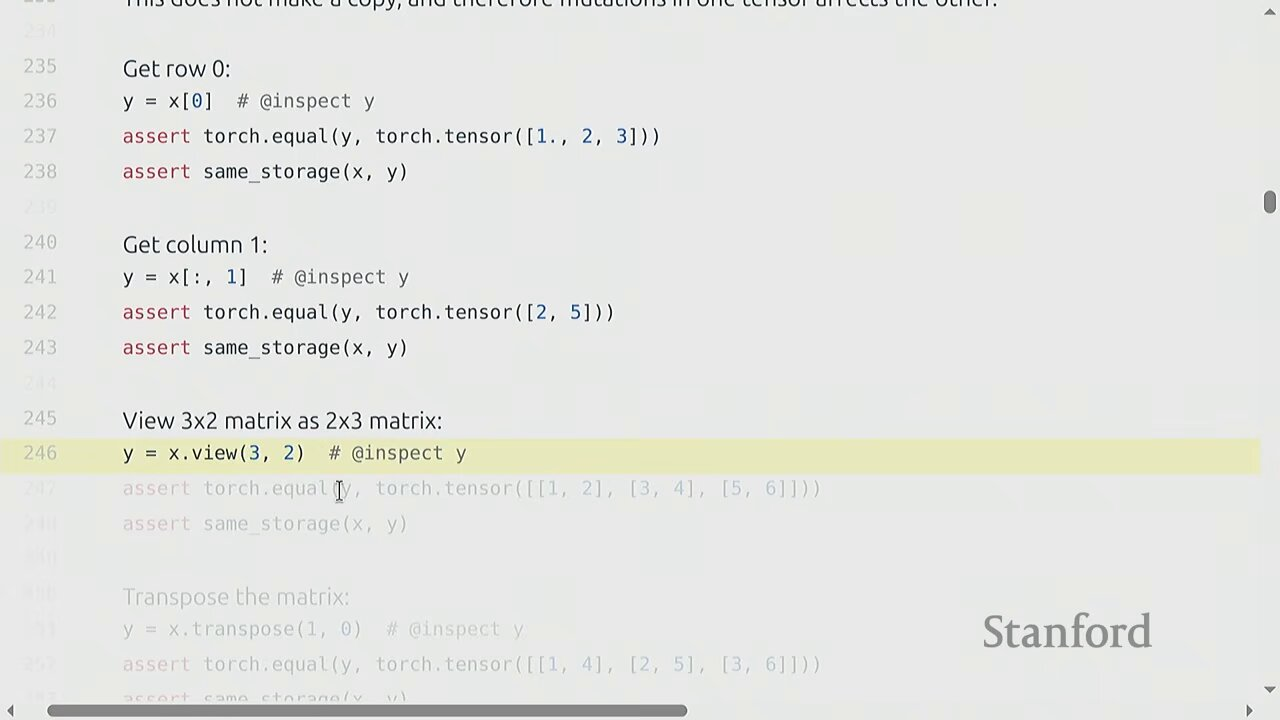
\includegraphics[width=\textwidth]{figures/fig_07_views_strides.jpg}
\caption{Views 与 strides：reshape/view 不拷贝数据，仅改变逻辑形状与遍历步幅\protect\footnotemark}
\end{figure}
\footnotetext{视频画面时间区间：20:45--21:15。}

\textbf{Strides} 是一个元组，告诉你"在某个维度上前进一个位置需要在底层一维存储里跳过多少个元素"。例如一个 row-major（行主序）的 $2 \times 3$ tensor，strides 是 $(3, 1)$：行方向前进 1 跳 3 个元素，列方向前进 1 跳 1 个元素。很多操作（transpose、reshape、slice）只改变 shape 和 strides，\textbf{不拷贝数据}——这叫 \texttt{view}。

\begin{figure}[H]
\centering
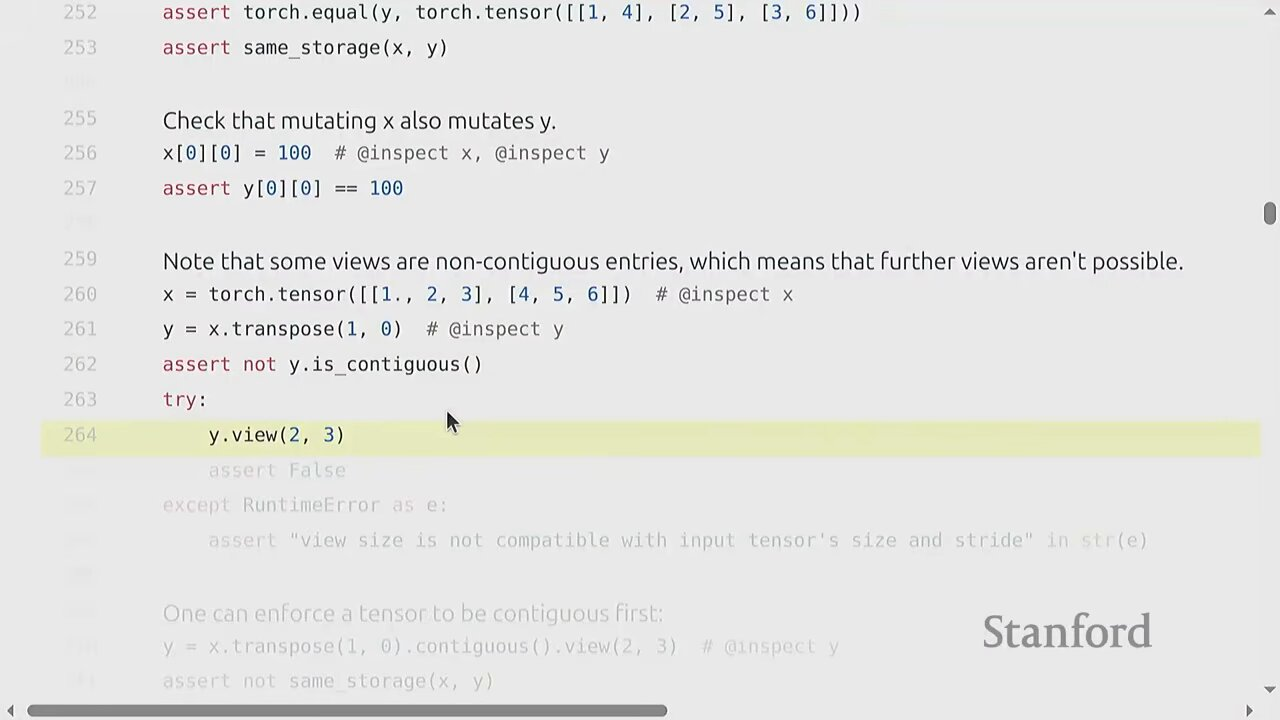
\includegraphics[width=\textwidth]{figures/fig_08_contiguous.jpg}
\caption{Contiguous tensors：view() 需连续内存，reshape() 总能用\protect\footnotemark}
\end{figure}
\footnotetext{视频画面时间区间：21:45--22:15。}

\begin{importantbox}{view() vs reshape()}
\begin{itemize}
\item \texttt{tensor.view(...)}：要求 tensor 是 \textbf{contiguous}（连续的），即元素在内存中按遍历顺序紧凑排列，否则报错。
\item \texttt{tensor.reshape(...)}：\textbf{总是可用}。如果不能做 view，它会自动拷贝数据。
\item 经验法则：想安全就 reshape；想确保不拷贝、对性能敏感就用 view（并在必要时先调 \texttt{.contiguous()}）。
\end{itemize}
\end{importantbox}

Percy 强调，理解 strides 能让你读懂那些看起来很"魔法"的代码（比如 \texttt{x[:, :-1]} 与 \texttt{x[:, 1:]} 共享底层存储），也能帮你调试奇怪的形状错误。

\subsection{ Broadcasting}

当两个 tensor 形状不同但要做逐元素运算时，PyTorch 用 \textbf{broadcasting}（广播）规则自动扩展较小的 tensor。规则是：从右向左对齐维度，每个维度要么相等、要么其中一个是 1（被扩展）、要么不存在（被当作 1）。这让代码更简洁，但也容易引入隐蔽的 bug——Percy 提醒要养成对每个 tensor 标注维度含义的习惯。

\section{计算图与 Autograd}

\subsection{Autograd：自动微分}

\begin{figure}[H]
\centering
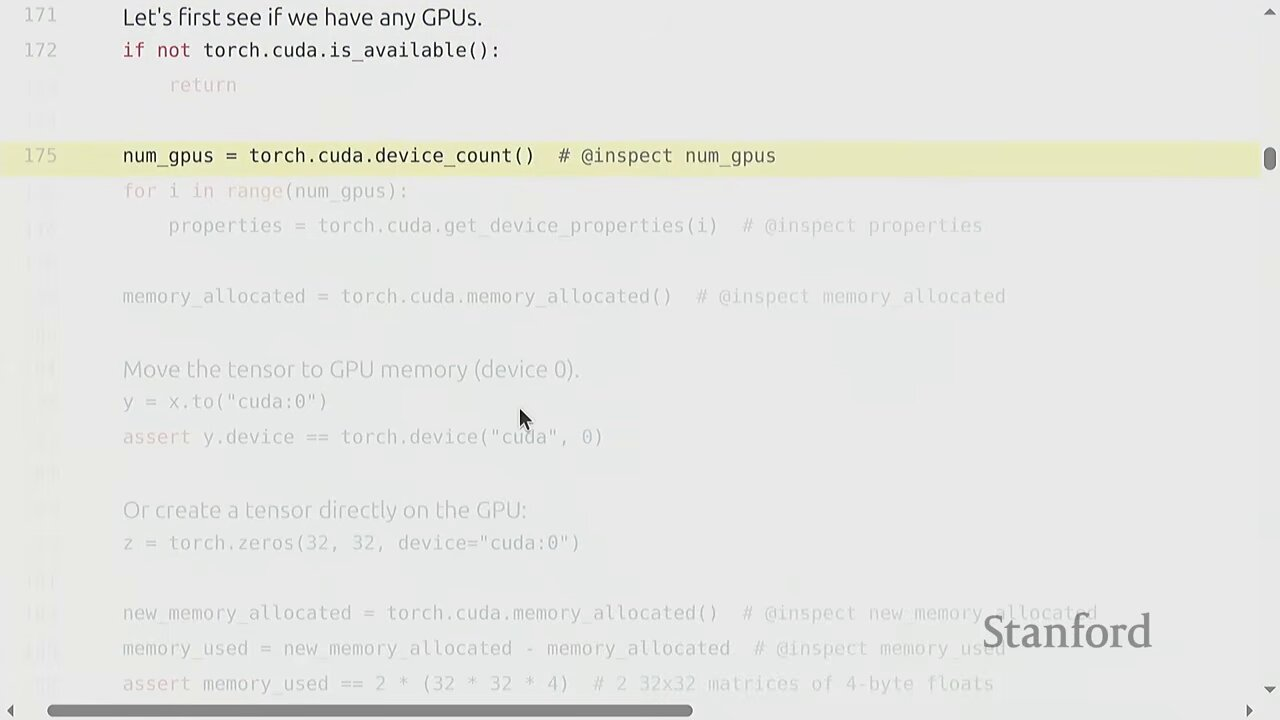
\includegraphics[width=\textwidth]{figures/fig_09_autograd.jpg}
\caption{Autograd：requires\_grad=True + backward() 自动计算梯度\protect\footnotemark}
\end{figure}
\footnotetext{视频画面时间区间：15:45--16:15。}

Percy 现场提醒一个常见误区：\texttt{backward()} 默认只释放计算图、保留叶节点的梯度。如果你想在非叶节点上检查中间梯度（用于调试），必须显式调用 \texttt{tensor.retain\_grad()}，否则反向传播一过该节点，它的梯度就被丢弃以节省内存。理解这一点能帮你解释"为什么打印某个中间变量的 \texttt{.grad} 却得到 \texttt{None}"。

PyTorch 的 \textbf{autograd}（自动微分引擎）是深度学习的核心。机制很简单：

\begin{enumerate}
\item 创建 tensor 时设 \texttt{requires\_grad=True}，PyTorch 开始追踪对它的所有操作
\item 对这些操作，autograd 在后台构建一个 \textbf{computational graph}（计算图），记录每个操作及其反向求导方式
\item 调用 \texttt{loss.backward()} 后，autograd 沿计算图反向传播，用链式法则（chain rule）算出每个叶节点的梯度，存入 \texttt{tensor.grad}
\end{enumerate}

例如 \texttt{y = x ** 2; y.backward()} 后，\texttt{x.grad} 就是 $\frac{dy}{dx} = 2x$。

\subsection{计算图：leaf variables}

\begin{figure}[H]
\centering
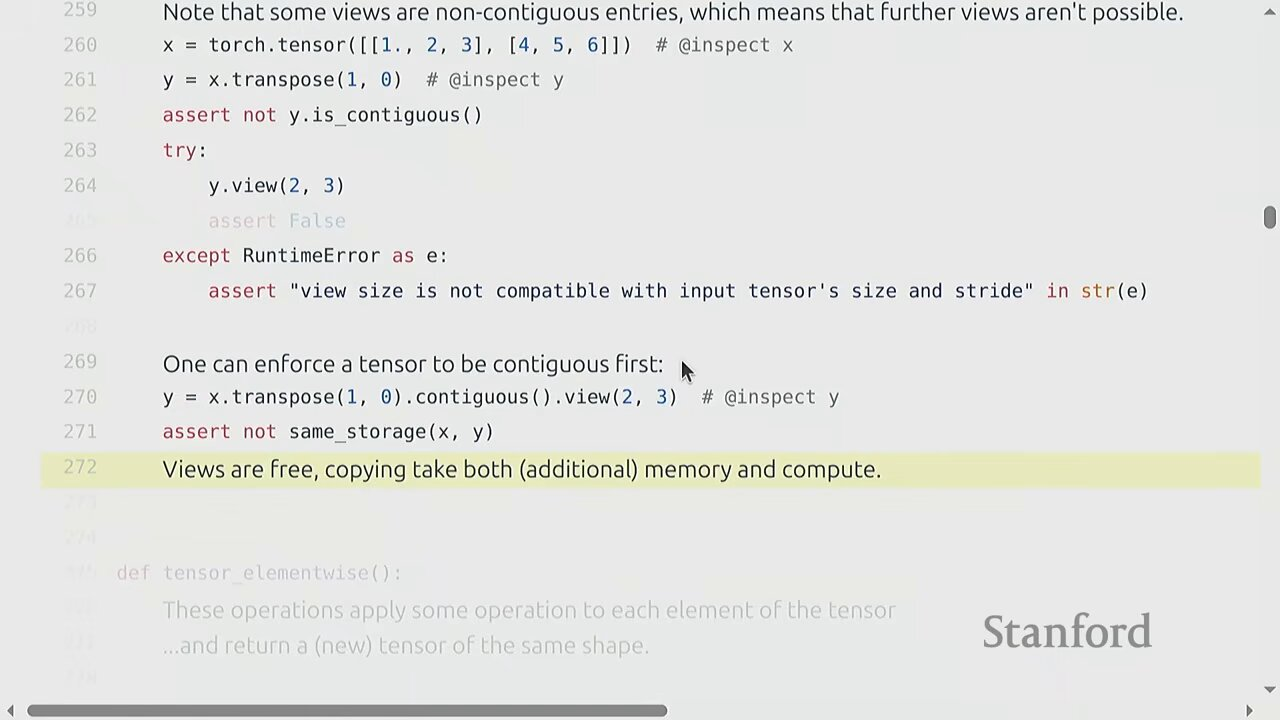
\includegraphics[width=\textwidth]{figures/fig_10_computational_graph.jpg}
\caption{计算图：leaf variables（用户创建的）与非叶子节点（操作产生的）\protect\footnotemark}
\end{figure}
\footnotetext{视频画面时间区间：22:45--23:15。}

计算图中的节点分两类。\textbf{Leaf variables}（叶变量）是用户直接创建的 tensor（如权重 $W$、输入 $x$），是梯度真正需要保留的目标。\textbf{非叶子节点}是操作产生的中间结果（如 $h = Wx$），它们的梯度在反向传播中被消费、默认不保留（节省内存）。如果想保留中间梯度，需调 \texttt{.retain\_grad()}。

\begin{knowledgebox}{为什么这样设计}
你真正要更新的是参数（叶变量），中间激活只是链式法则的"过路费"。默认丢弃中间梯度是内存优化。理解 leaf vs non-leaf 是排查"为什么我的 \texttt{.grad} 是 None"这类 bug 的关键。
\end{knowledgebox}

\section{构建模型：nn.Module}

\subsection{nn.Linear：最小的模块}

\begin{figure}[H]
\centering
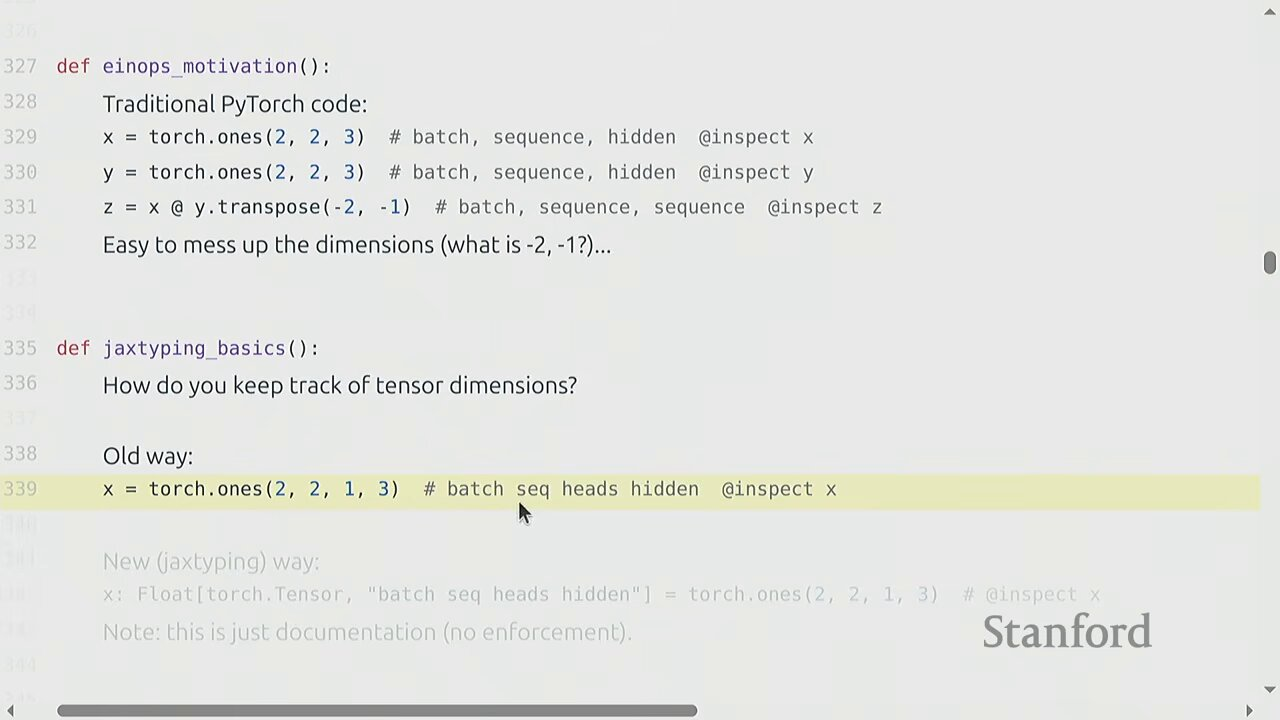
\includegraphics[width=\textwidth]{figures/fig_11_nn_linear.jpg}
\caption{nn.Linear：weight 是 Parameter，forward 做 F.linear(x, weight)\protect\footnotemark}
\end{figure}
\footnotetext{视频画面时间区间：26:45--27:15。}

\texttt{nn.Linear} 是最基础的模块。它持有一个权重矩阵 $W \in \mathbb{R}^{d_{\text{out}} \times d_{\text{in}}}$（PyTorch 约定这样存），\texttt{forward} 就是 $y = xW^\top$（加可选 bias）。关键点：$W$ 是 \texttt{nn.Parameter}——这是 \texttt{nn.Tensor} 的子类，会被自动注册为"需要求梯度的模块参数"，从而被 optimizer 发现和更新。

线性层的前向计算为：

\[
h = x W^\top, \quad x \in \mathbb{R}^{B \times d_{\text{in}}}, \; W \in \mathbb{R}^{d_{\text{out}} \times d_{\text{in}}}, \; h \in \mathbb{R}^{B \times d_{\text{out}}}
\]

\begin{itemize}
\item $x$：输入，形状 $(B, d_{\text{in}})$，$B$ 为 batch（或 batch $\times$ sequence）
\item $W$：权重，形状 $(d_{\text{out}}, d_{\text{in}})$，是可学习参数
\item $h$：输出，形状 $(B, d_{\text{out}})$
\end{itemize}

\subsection{nn.Module：组合的基石}

\begin{figure}[H]
\centering
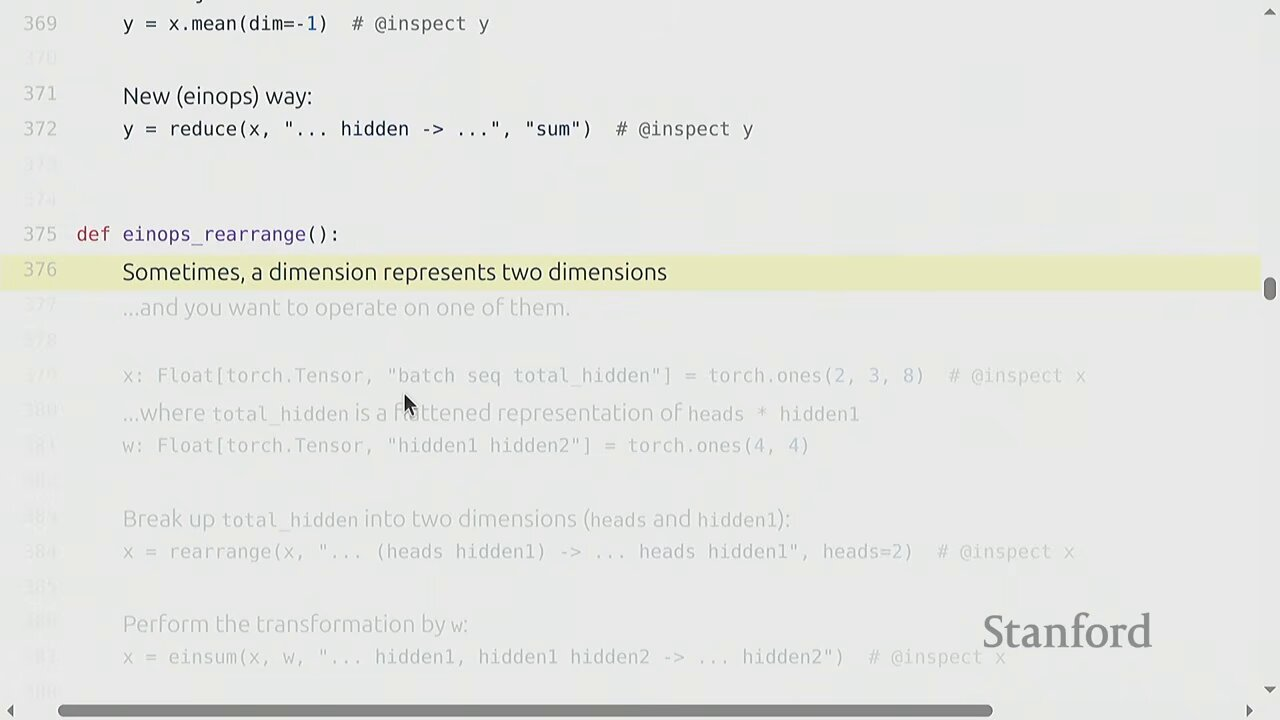
\includegraphics[width=\textwidth]{figures/fig_12_mlp_module.jpg}
\caption{MLP 的 nn.Module 实现：\_\_init\_\_ 定义子层，forward 描述计算\protect\footnotemark}
\end{figure}
\footnotetext{视频画面时间区间：30:45--31:15。}

\texttt{nn.Module} 是所有模型组件的基类。它的两个核心方法：

\begin{itemize}
\item \texttt{\_\_init\_\_(self, ...)}：声明子模块和参数（如 \texttt{self.fc1 = nn.Linear(...)}）
\item \texttt{forward(self, x)}：描述前向计算流程
\end{itemize}

\texttt{nn.Module} 自动追踪所有子模块和参数（通过 \texttt{.parameters()} 迭代器暴露给 optimizer）。一个两层 MLP（Linear $\to$ ReLU $\to$ Linear $\to$ ReLU）就是 \texttt{nn.Module} 的典型用法。这种"声明 + forward"的模式让模型定义既模块化又可读。

\subsection{Einsum：给维度起名字}

PyTorch 代码里常见 \texttt{x @ y.transpose(-2, -1)} 这种用 $-2, -1$ 索引维度的写法，很容易出错且难读。Percy 推荐用 \textbf{einsum}（爱因斯坦求和约定，Einstein summation notation）和 \texttt{jaxtyping} 库来给维度命名。例如：

\[
\texttt{torch.einsum("bs h, b s k h -> b s k", x, y)}
\]

直接写出 batch（b）、sequence（s）、hidden（h）等维度名。einsum 的规则：输出里出现的维度被遍历，没出现的维度被求和。虽然初看冗长，但比 $-2, -1$ 更不易错，也便于文档化。\texttt{jaxtyping} 进一步用类型注解强制维度一致性（但 PyTorch 默认不强制，需额外 checker）。

Percy 还提到一个实用技巧：用 \texttt{...}（省略号）表示"广播任意数量的前导维度"，这样写出的 einsum 更紧凑、更通用。例如 \texttt{"... s h, ... s h -> ... s"} 可以同时处理带或不带 batch 维度的输入。养成给维度命名的习惯，能让你的代码在面对 batch、sequence、head 等多维 tensor 时少出低级形状错误。

\subsection{训练循环}

\begin{figure}[H]
\centering
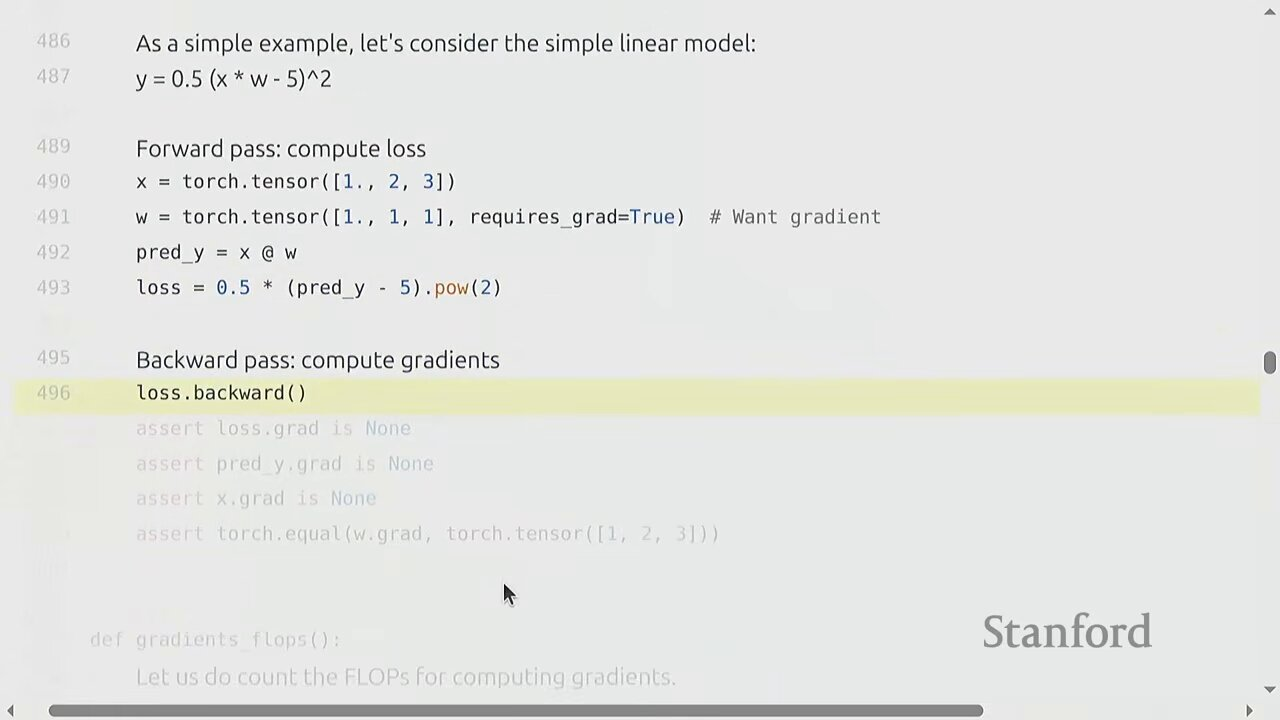
\includegraphics[width=\textwidth]{figures/fig_13_training_loop.jpg}
\caption{标准训练循环：forward $\to$ loss $\to$ zero\_grad $\to$ backward $\to$ step\protect\footnotemark}
\end{figure}
\footnotetext{视频画面时间区间：50:45--51:15。}

一个标准的 PyTorch 训练循环骨架如下：

\begin{lstlisting}[language=Python]
for batch in dataloader:
    inputs, labels = batch
    outputs = model(inputs)          # 前向
    loss = criterion(outputs, labels)  # 算 loss
    optimizer.zero_grad()            # 清上轮梯度
    loss.backward()                  # 反向传播
    optimizer.step()                 # 更新参数
\end{lstlisting}

\begin{warningbox}{容易忘的 zero\_grad()}
\texttt{optimizer.zero\_grad()} 必须在每次 \texttt{backward()} 前调用。因为 PyTorch 默认把新梯度\textbf{累加}到 \texttt{.grad} 上（这是 gradient accumulation 的基础）。如果你忘了清零，梯度会一直累加，训练立刻发散。
\end{warningbox}

\section{算力核算：从 matmul 到 6ND}

\subsection{矩阵乘法的 FLOPs}

\begin{figure}[H]
\centering
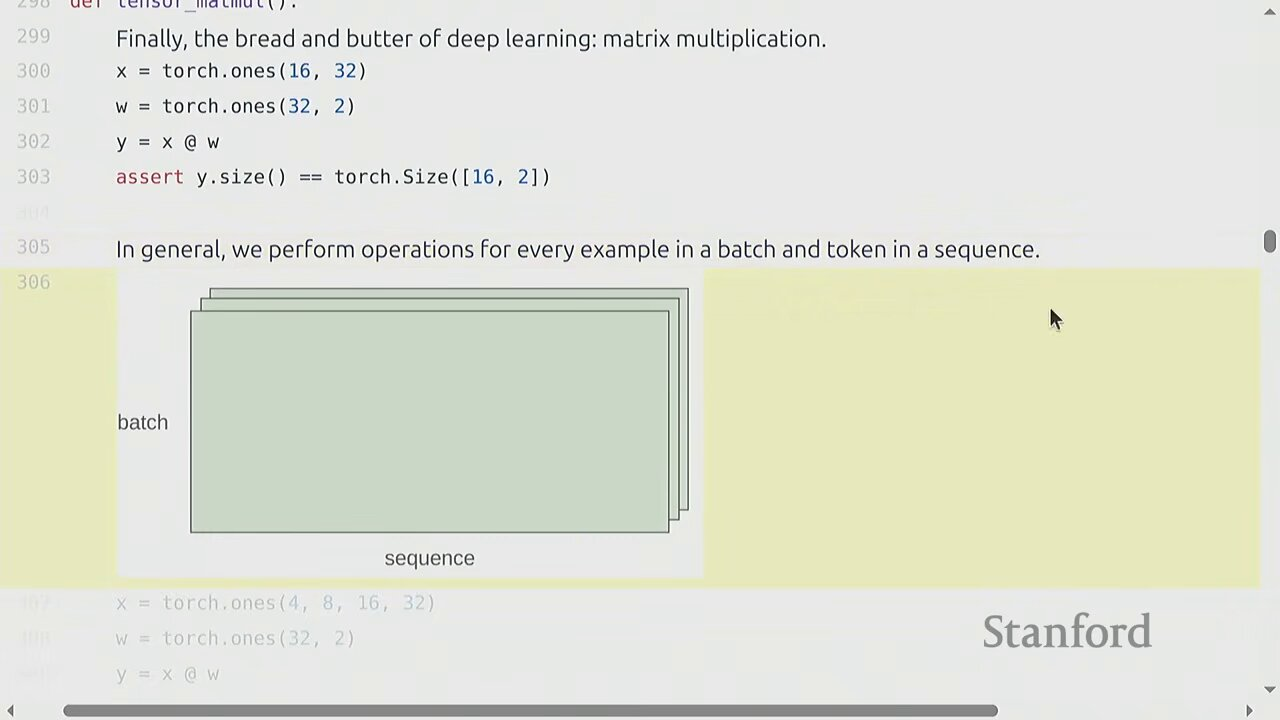
\includegraphics[width=\textwidth]{figures/fig_14_matmul_flops.jpg}
\caption{矩阵乘法 FLOPs：$C = AB$，$(m \times k)(k \times n)$，总 FLOPs $= 2mnk$\protect\footnotemark}
\end{figure}
\footnotetext{视频画面时间区间：24:15--24:45。}

矩阵乘法（matmul）是深度学习的"面包黄油"。$C = AB$，其中 $A \in \mathbb{R}^{m \times k}$、$B \in \mathbb{R}^{k \times n}$、$C \in \mathbb{R}^{m \times n}$。$C$ 的每个元素是 $A$ 的一行与 $B$ 的一列的点积，需要 $k$ 次乘法和 $k-1$ 次加法 $\approx 2k$ 次 FLOPs。$C$ 共 $mn$ 个元素，所以：

\[
\text{FLOPs}_{\text{matmul}} = 2 \cdot m \cdot n \cdot k
\]

\begin{itemize}
\item $m, n, k$：两个矩阵的三个维度
\item 系数 2：每次乘加算作 2 次 FLOPs（1 乘 + 1 加）
\item 这条 "$2 \times$ 所有维度乘积" 的规则是后续所有算力核算的基础
\end{itemize}

在语言模型里，matmul 通常带 batch 和 sequence 维度（$B \times S \times \dots$），但规则不变——每个 batch、每个 token 独立做 matmul，总 FLOPs 就是再乘上 $B \cdot S$。

\subsection{从 matmul 到 FLOPs/s 再到 MFU}

\begin{figure}[H]
\centering
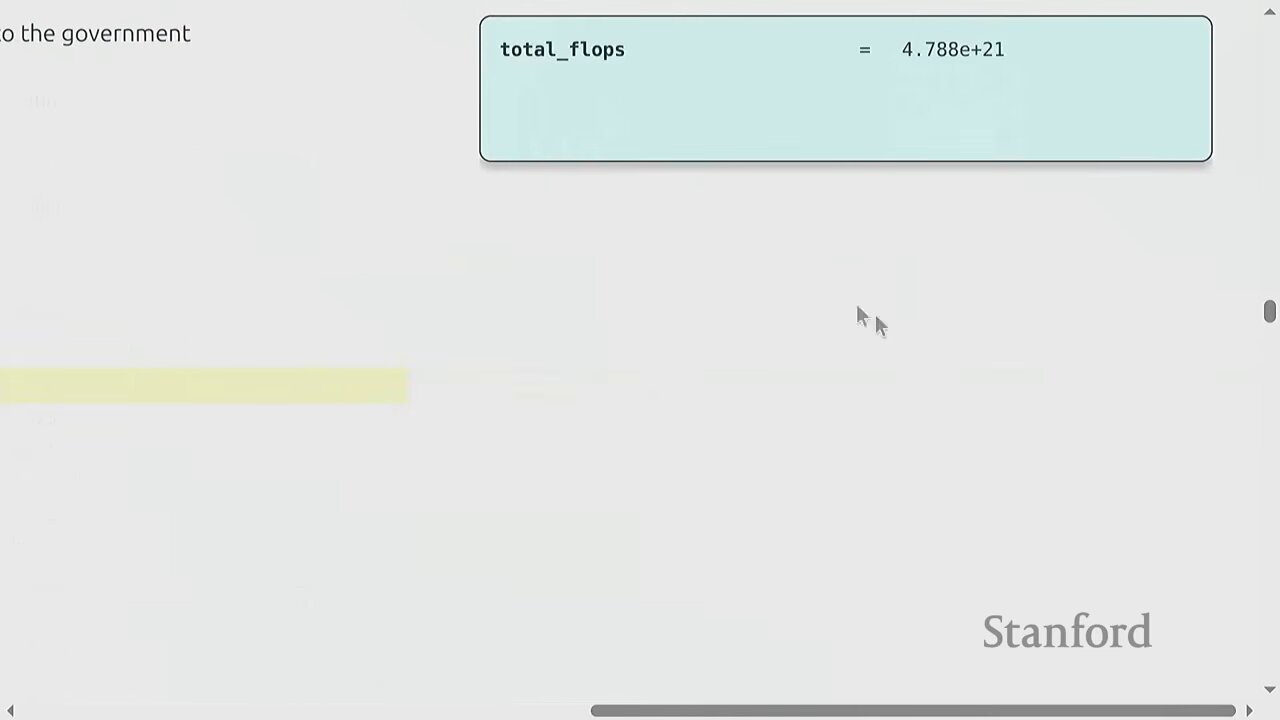
\includegraphics[width=\textwidth]{figures/fig_22_h100_tflops.jpg}
\caption{H100 峰值算力与每天秒数：989 TFLOPS（BF16），每天 86400 秒\protect\footnotemark}
\end{figure}
\footnotetext{视频画面时间区间：36:45--37:15。}

知道了某个 matmul 的 FLOPs，再用 \texttt{time} 模块测它实际耗时，就能得到实际吞吐：

\[
\text{actual FLOPs/s} = \frac{\text{FLOPs}_{\text{matmul}}}{\text{wall\_time}}
\]

把这个数和硬件的"宣传峰值"对比，就得到 \textbf{MFU}（model FLOPs utilization，模型算力利用率）：

\[
\text{MFU} = \frac{\text{actual FLOPs/s}}{\text{promised FLOPs/s}}
\]

\begin{itemize}
\item $\text{actual FLOPs/s}$：你实测的吞吐（模型有效计算量 / 实际耗时）
\item $\text{promised FLOPs/s}$：硬件宣传的峰值（如 H100 的 989 TFLOPS BF16），来自厂家"光面宣传册"
\item 注意：MFU 看的是\textbf{模型的有效计算量}，不是硬件实际执行的指令数——所以即使你用了 gradient checkpointing 多算了一遍前向，MFU 仍按"模型本该算的量"计，不会因为你"聪明"而惩罚你
\end{itemize}

\begin{importantbox}{MFU 的经验值}
\begin{itemize}
\item MFU $> 0.5$：通常被认为是"好"的实现
\item MFU $\approx 0.05$（5\%）：很差，说明有大把算力被浪费在通信、kernel 启动、内存搬运上
\item 几乎不可能达到 0.9--1.0，因为这忽略了所有通信和开销，只算纯计算
\item matmul 占主导时 MFU 通常更高
\item \textbf{永远要 benchmark 你的代码}，别假设能拿到宣传峰值
\end{itemize}
\end{importantbox}

\begin{figure}[H]
\centering
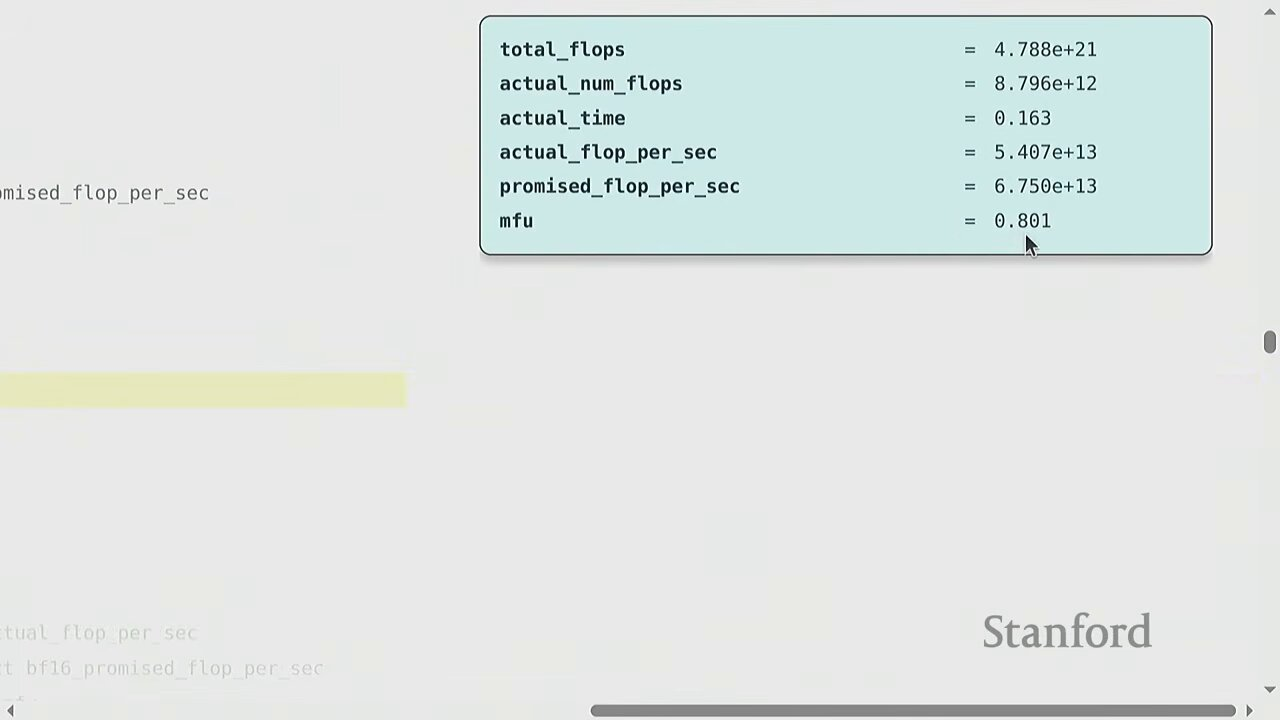
\includegraphics[width=\textwidth]{figures/fig_21_training_time.jpg}
\caption{训练时间估算完整公式：$6 \times 70\text{B} \times 15\text{T} / (1024 \times 989\text{e}12 \times 0.5 \times 86400) \approx 144$ 天\protect\footnotemark}
\end{figure}
\footnotetext{视频画面时间区间：44:45--45:15。}

把 MFU 串进来，训练时间的完整公式为：

\[
T_{\text{train}} = \frac{6 \cdot N \cdot D}{G \cdot P \cdot \text{MFU}}
\]

\begin{itemize}
\item $N$：模型参数量，$D$：训练 token 数
\item 分子 $6ND$：总训练 FLOPs（前向 2 + 反向 4，下节推导）
\item $G$：GPU 数量，$P$：单卡峰值 FLOPs/s
\item 代入开场问题：$N=70\text{B}, D=15\text{T}, G=1024, P=989\text{e}12, \text{MFU}=0.5$，得 $\approx 144$ 天
\end{itemize}

\begin{knowledgebox}{Tensor Core 与 BF16 的关系}
学生提问：PyTorch 默认会用 tensor core 吗？答案是：tensor core 是 GPU 上专门做 matmul 的硬件单元，spec sheet 上那些高 FLOPs 数字\textbf{都是基于 tensor core 的}。用 BF16/F16 且配合 \texttt{torch.compile}，PyTorch 会生成调用 tensor core 的代码。FP32 路径的峰值则低得多（如 H100 FP32 约 67 TFLOPS，BF16 约 989 TFLOPS）。
\end{knowledgebox}

\subsection{Linear Layer 的 FLOPs：前向与反向}

\begin{figure}[H]
\centering
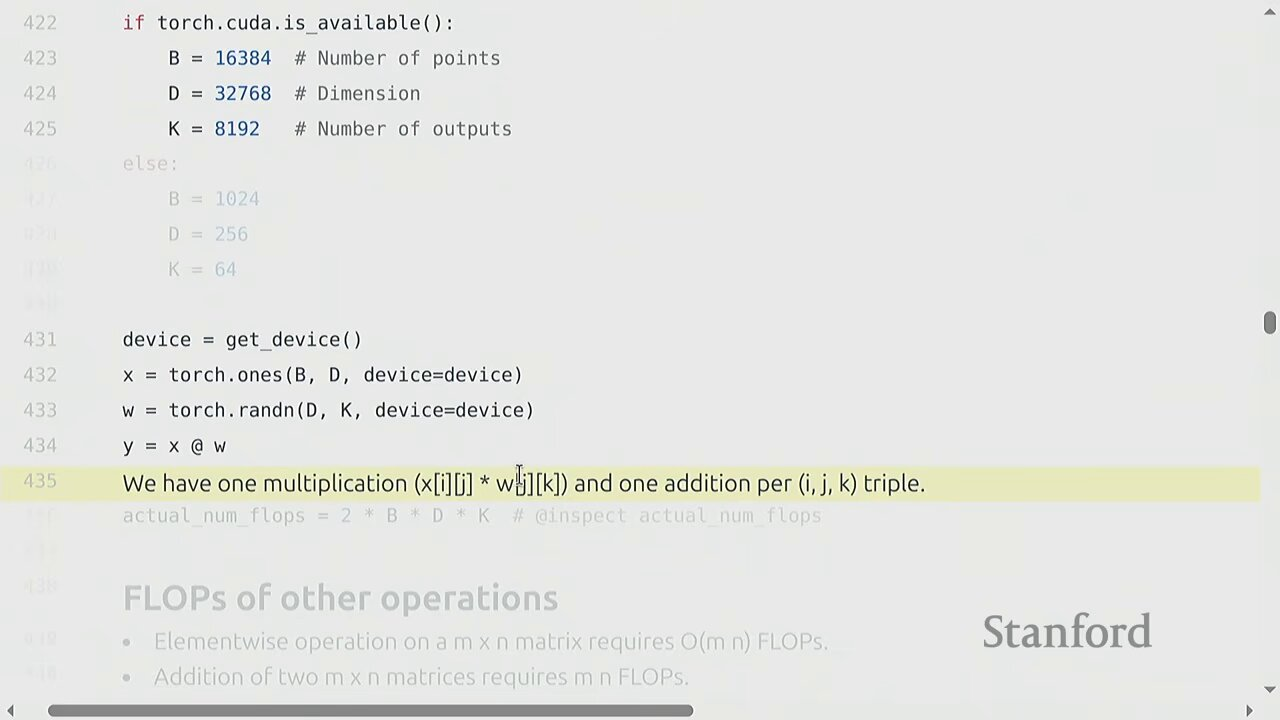
\includegraphics[width=\textwidth]{figures/fig_15_linear_flops.jpg}
\caption{Linear layer FLOPs：单 token 前向 $2d_{\text{in}}d_{\text{out}}$，反向约 $4d_{\text{in}}d_{\text{out}}$\protect\footnotemark}
\end{figure}
\footnotetext{视频画面时间区间：38:45--39:15。}

考虑一个两层线性网络：$H_1 = X W_1$（$X \in \mathbb{R}^{B \times D}$，$W_1 \in \mathbb{R}^{D \times D}$），$H_2 = H_1 W_2$（$W_2 \in \mathbb{R}^{D \times K}$），再算 loss。

\subsubsection{前向 FLOPs}

前向就是两个 matmul：

\[
\text{FLOPs}_{\text{fwd}} = 2 \cdot B \cdot D \cdot D + 2 \cdot B \cdot D \cdot K = 2 \cdot B \cdot (\text{参数量})
\]

\begin{itemize}
\item 第一项 $2BDD$：$X W_1$，对应 $W_1$ 的 $D \cdot D$ 个参数
\item 第二项 $2BDK$：$H_1 W_2$，对应 $W_2$ 的 $D \cdot K$ 个参数
\item 关键观察：\textbf{前向 FLOPs $= 2 \times$ batch $\times$ 参数量}
\end{itemize}

\subsubsection{反向 FLOPs：链式法则}

反向传播要算 $\partial \text{loss} / \partial W_1, \partial \text{loss} / \partial W_2, \partial \text{loss} / \partial H_1, \dots$。以 $W_2$ 为例，链式法则给出：

\[
\frac{\partial \text{loss}}{\partial W_2} = H_1^\top \frac{\partial \text{loss}}{\partial H_2}
\]

这本身是一个 matmul，FLOPs 为 $2 B D K$。但还要继续往前传 $\partial \text{loss} / \partial H_1$：

\[
\frac{\partial \text{loss}}{\partial H_1} = \frac{\partial \text{loss}}{\partial H_2} W_2^\top
\]

这又是一个 matmul，FLOPs 也是 $2 B D K$。所以仅 $W_2$ 这一层反向就需要 $2 \times 2BDK = 4BDK$。同理 $W_1$ 层反向需要 $4BDD$。

\begin{importantbox}{前向 2，反向 4，总共 6}
\[
\text{FLOPs}_{\text{fwd}} = 2 \cdot B \cdot (\text{参数量}), \quad \text{FLOPs}_{\text{bwd}} = 4 \cdot B \cdot (\text{参数量})
\]
\[
\text{FLOPs}_{\text{total}} = 6 \cdot B \cdot (\text{参数量})
\]
\begin{itemize}
\item 前向每个参数对应 $\approx 2$ FLOPs（一次 matmul）
\item 反向每个参数对应 $\approx 4$ FLOPs（两个 matmul：算 $\partial/\partial W$ 和 $\partial/\partial H$）
\item 总计 $6 \times$ 参数量 $\times$ 数据点数——这正是开场公式 $6ND$ 中 6 的来源
\end{itemize}
\end{importantbox}

\subsubsection{推广到 Transformer}

\begin{figure}[H]
\centering
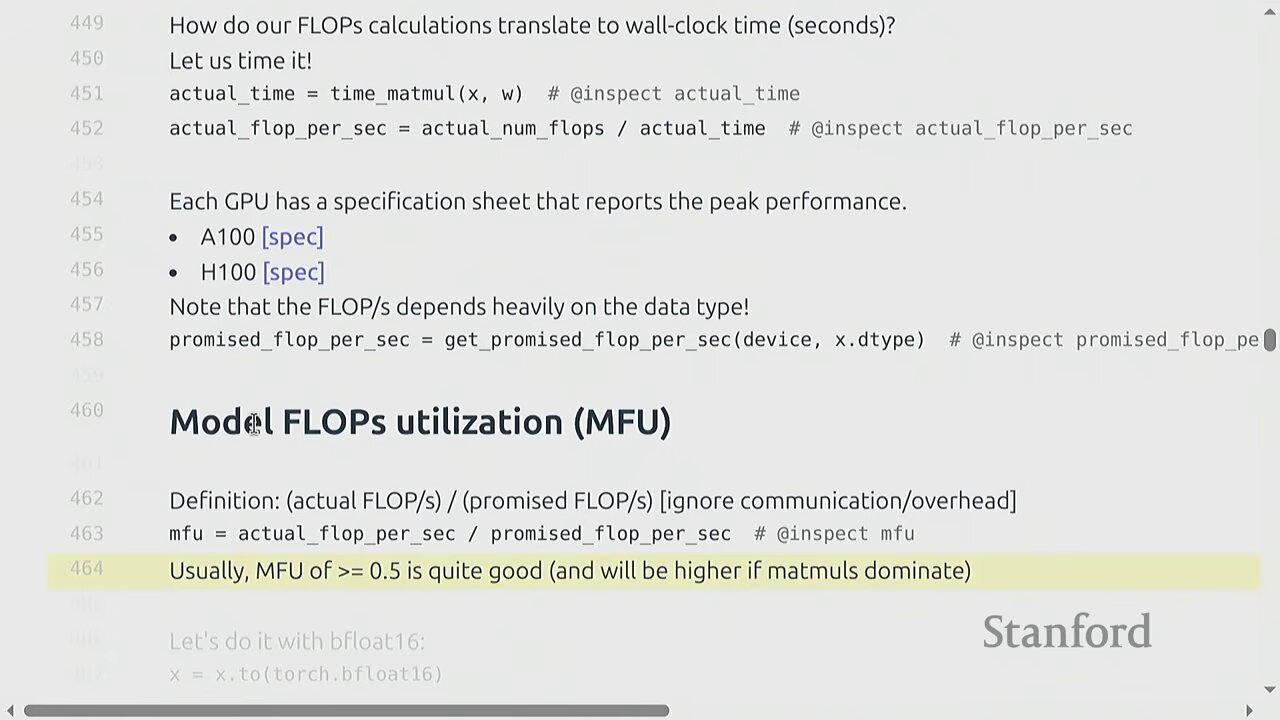
\includegraphics[width=\textwidth]{figures/fig_17_transformer_6nd.jpg}
\caption{Transformer 训练总 FLOPs $\approx 6ND$：6 的来源是前向 2 + 反向 4\protect\footnotemark}
\end{figure}
\footnotetext{视频画面时间区间：46:45--47:15。}

这个 $6 \times$ 规则对绝大多数模型成立，因为大部分计算都是 matmul，且每个计算大致"触及"一组新参数。例外是参数共享（如一个参数被复用亿次，FLOPs 远超 $6N$），但正常模型不这样。因此 Transformer 的训练 FLOPs 也近似为：

\[
\text{FLOPs}_{\text{transformer}} \approx 6 \cdot N_{\text{params}} \cdot N_{\text{tokens}}
\]

\subsection{Attention 的 FLOPs}

\begin{figure}[H]
\centering
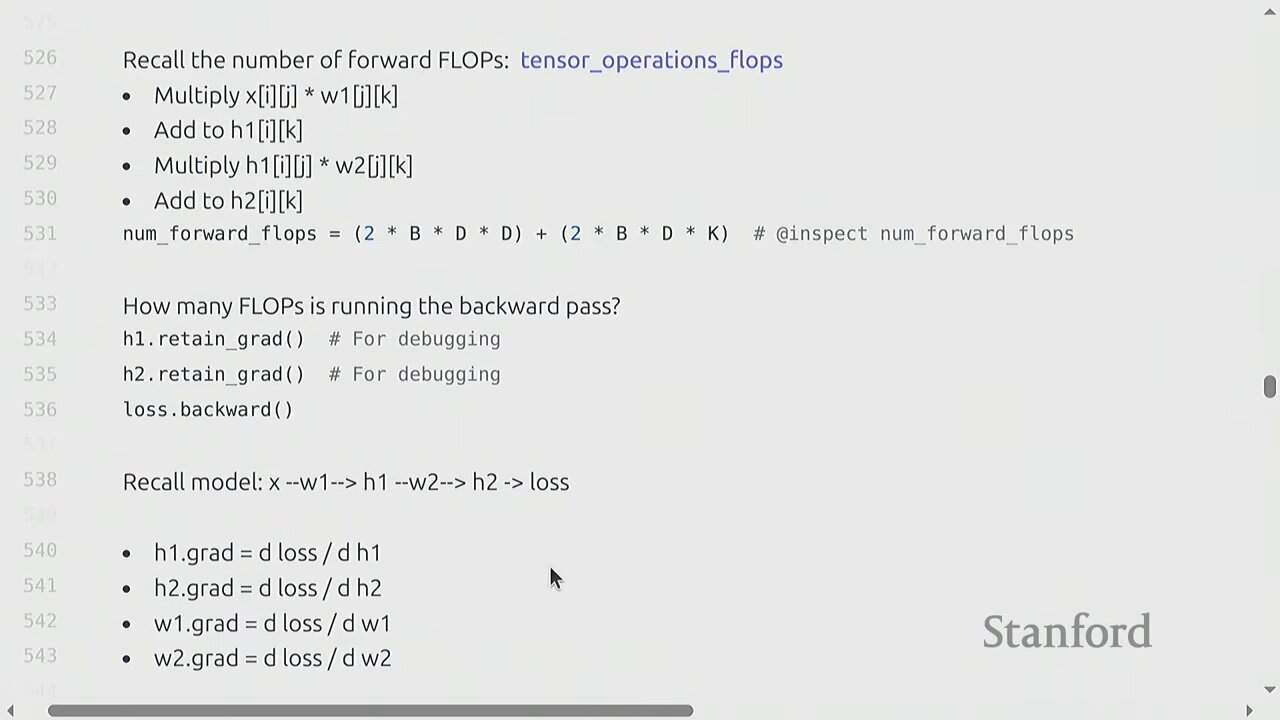
\includegraphics[width=\textwidth]{figures/fig_16_attention_flops.jpg}
\caption{Attention FLOPs：$\text{softmax}(QK^\top/\sqrt{d})V$，QKV 投影主导计算量\protect\footnotemark}
\end{figure}
\footnotetext{视频画面时间区间：54:45--55:15。}

标准 attention 的计算为：

\[
\text{Attention}(Q, K, V) = \text{softmax}\left(\frac{Q K^\top}{\sqrt{d_k}}\right) V
\]

FLOPs 分解：
\begin{itemize}
\item $QK^\top$：$(B \times S \times d) \times (B \times d \times S) \to (B \times S \times S)$，FLOPs $= 2 B S^2 d$
\item $\text{softmax}(QK^\top) V$：$(B \times S \times S) \times (B \times S \times d) \to (B \times S \times d)$，FLOPs $= 2 B S^2 d$
\item softmax 本身的 FLOPs 相对可忽略
\item 还有 $Q, K, V$ 三个投影和输出投影，每个是 $2 B S d^2$
\end{itemize}

\begin{knowledgebox}{Attention 的两个 regimes}
当序列长度 $S$ 远小于隐藏维度 $d$ 时，$QKV$ 投影（$O(Sd^2)$）主导；当 $S$ 很大时，$QK^\top$ 和 $\text{softmax} V$（$O(S^2 d)$）主导——这正是长序列的瓶颈，催生了 FlashAttention、sliding window 等优化。在第一讲提到的 175B 模型上，MLP 的 FLOPs 占主导（约 2/3），attention 相对小。
\end{knowledgebox}

\section{内存核算：四类占用}

讲完算力，回到内存。一个训练中的模型，内存被四类对象占用。

\subsection{参数与梯度}

\textbf{Parameters}（参数）：模型权重本身。对一个 $L$ 层、隐藏维度 $d$ 的简单模型，参数量约为 $L \cdot d^2 + d$（最后一层 head 是 $d$）。

\textbf{Gradients}（梯度）：与参数一一对应，\textbf{形状和数量完全相同}。所以梯度占用 $=$ 参数占用。

\subsection{激活内存}

\begin{figure}[H]
\centering
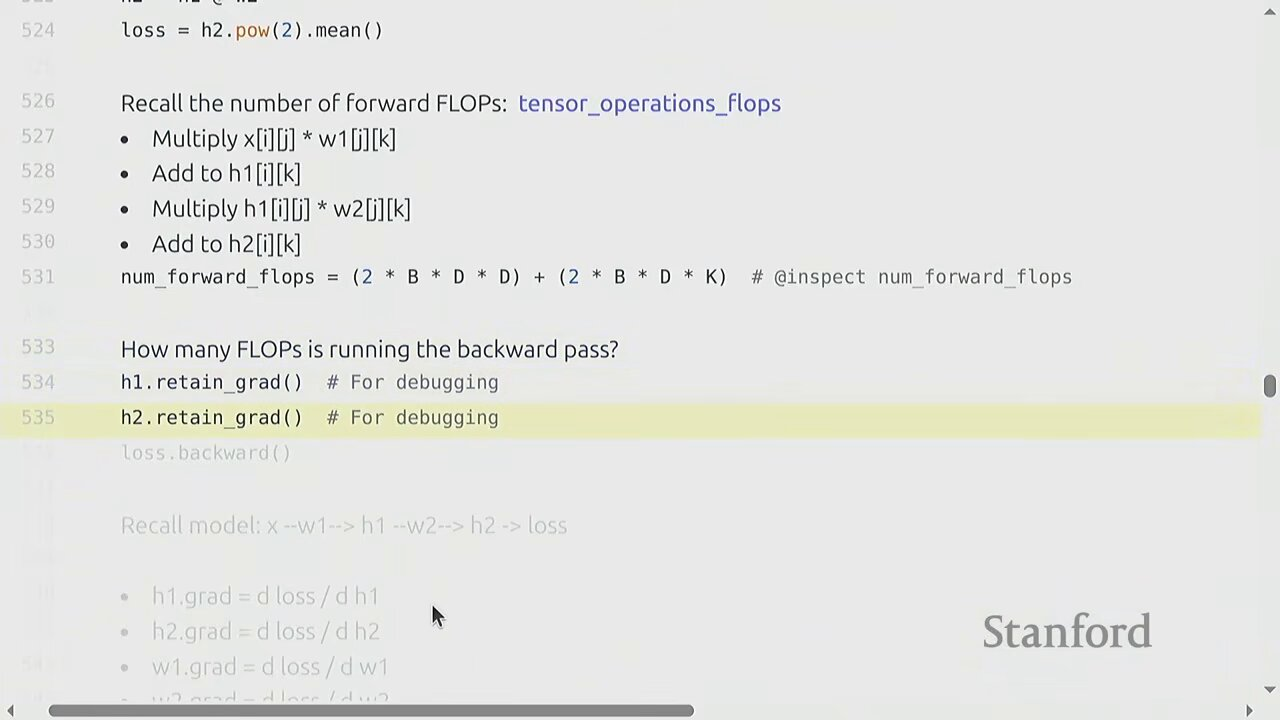
\includegraphics[width=\textwidth]{figures/fig_18_activation_memory.jpg}
\caption{激活内存：随层数线性增长，每层激活需缓存供反向传播\protect\footnotemark}
\end{figure}
\footnotetext{视频画面时间区间：52:45--53:15。}

\textbf{Activations}（激活）：反向传播时，第 $i$ 层的梯度依赖于第 $i$ 层的输入激活。所以前向时必须\textbf{把每层激活缓存下来}，留到反向时用。激活占用为：

\[
\text{memory}_{\text{act}} = B \cdot S \cdot d \cdot L \cdot (\text{bytes\_per\_element})
\]

\begin{itemize}
\item $B$：batch size，$S$：序列长度，$d$：隐藏维度，$L$：层数
\item 每个数据点、每个 token、每层都要存一个 $d$ 维向量
\item \textbf{激活内存随层数 $L$ 线性增长}——这是深层模型的主要内存瓶颈
\end{itemize}

\begin{warningbox}{为什么要存激活}
反向传播算第 $i$ 层权重的梯度需要第 $i$ 层的输入。朴素做法是全存下来。但有更聪明的办法——下节的 gradient checkpointing。
\end{warningbox}

\subsection{优化器状态内存}

\begin{figure}[H]
\centering
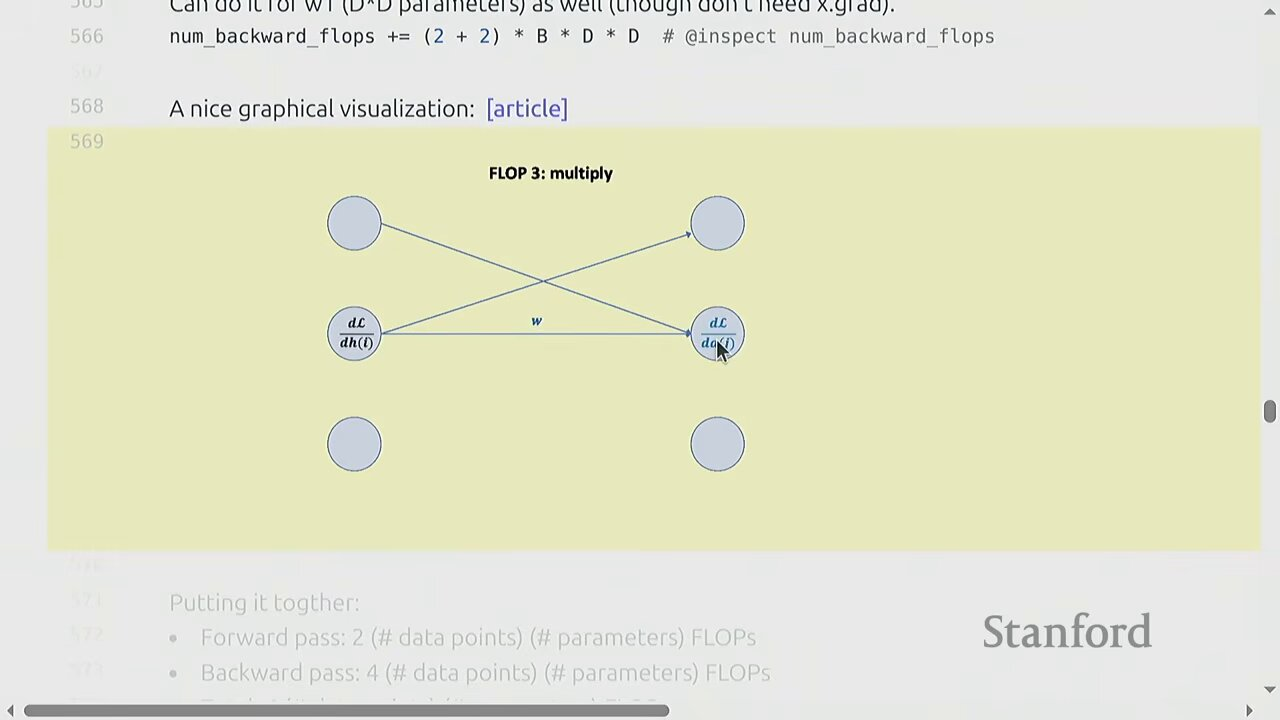
\includegraphics[width=\textwidth]{figures/fig_20_optimizer_memory.jpg}
\caption{优化器状态内存：AdamW 需存 $m$ 和 $v$（各 FP32），每参数约 12--16 字节\protect\footnotemark}
\end{figure}
\footnotetext{视频画面时间区间：56:45--57:15。}

\textbf{Optimizer state}（优化器状态）：这是最容易被忽略、却往往占用最大的一块。不同优化器状态量不同：

\begin{tabular}{p{2.5cm}p{3cm}p{8cm}}
\toprule
\textbf{优化器} & \textbf{状态量（每参数）} & \textbf{说明} \\
\midrule
SGD（无 momentum） & 0 & 只用梯度，无额外状态 \\
SGD with momentum & 1 份（velocity $v$） & 累加梯度的滑动平均 \\
Adagrad & 1 份（$G = \sum g^2$） & 累加历史梯度平方和 \\
RMSprop & 1 份（$E[g^2]$） & Adagrad 的指数衰减版 \\
Adam / AdamW & 2 份（$m$ 和 $v$） & 一阶矩 + 二阶矩的指数滑动平均 \\
\bottomrule
\end{tabular}

\begin{importantbox}{AdamW 的每参数内存（FP32）}
\[
\text{bytes/param} = \underbrace{4}_{\text{param}} + \underbrace{4}_{\text{grad}} + \underbrace{4}_{m} + \underbrace{4}_{v} = 16 \text{ 字节}
\]
若用混合精度（参数存 BF16 但 optimizer state 存 FP32）：参数 2 + 梯度 2 + $m$ 4 + $v$ 4 $= 12$ 字节。这就是开场"16 字节/参数"和"8 张 H100 能训 40B"的由来。
\end{importantbox}

\subsection{总内存公式}

把四类加起来：

\[
\text{memory}_{\text{total}} = (\text{params} + \text{grads} + \text{optim\_state}) \times \text{bytes} + \text{activations}
\]

\begin{itemize}
\item 前三项正比于参数量 $N$，与 batch/sequence 无关
\item activations 正比于 $B \cdot S \cdot d \cdot L$，随 batch 和序列长度增长
\item Assignment 1 要求对 Transformer 做这个分解——形式相同，只是矩阵更多
\end{itemize}

Percy 用一个具体数字收尾这个例子：对一个 $d=2048$、$L=8$ 层、$B=64$ 的模型，参数部分约占几百兆字节，而激活部分也达到同样量级——这说明在中等规模下激活就已经和参数相当，深层大模型时激活甚至会超过参数。这也是为什么 gradient checkpointing、混合精度等技术如此重要：它们直接削减的是这四类占用中最大的一块。

\section{Optimizer 的实现}

\begin{figure}[H]
\centering
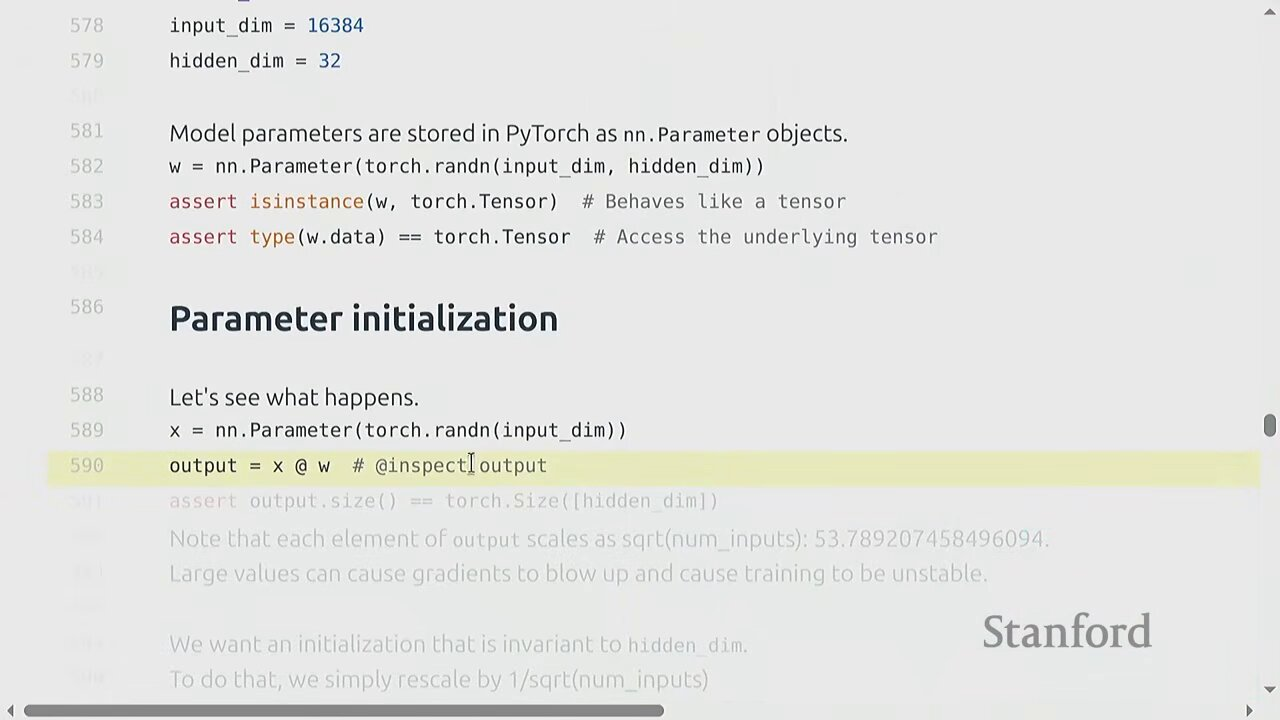
\includegraphics[width=\textwidth]{figures/fig_23_optimizer_summary.jpg}
\caption{优化器实现：继承 Optimizer，在 step() 里读梯度、更新状态、改参数\protect\footnotemark}
\end{figure}
\footnotetext{视频画面时间区间：60:45--61:15。}

在 PyTorch 里实现自定义 optimizer，需继承 \texttt{torch.optim.Optimizer} 并重写 \texttt{step()}。Percy 现场演示了 \textbf{Adagrad} 的实现（因为 Assignment 1 要实现 Adam，所以课上讲 Adagrad 避免剧透）。

\textbf{Adagrad} 的更新规则：维护一个累积量 $G = \sum_t g_t^2$（逐元素），更新时：

\[
G_t = G_{t-1} + g_t \odot g_t, \quad \theta_t = \theta_{t-1} - \frac{\eta}{\sqrt{G_t + \epsilon}} \odot g_t
\]

\begin{itemize}
\item $G_t$：历史梯度平方和（optimizer state，每个参数一份）
\item $g_t$：当前梯度（由 \texttt{backward()} 算好，存在 \texttt{param.grad}）
\item $\eta$：学习率，$\epsilon$：防除零小常数
\item $\odot$：逐元素乘除
\end{itemize}

\begin{knowledgebox}{优化器的演进谱系}
SGD $\to$ momentum（加滑动平均）$\to$ Adagrad（按参数自适应步长，但 $G$ 单调增导致步长趋零）$\to$ RMSprop（用指数衰减代替单调累加）$\to$ Adam（2014，结合 momentum + RMSprop，同时维护 $m$ 和 $v$）$\to$ AdamW（解耦 weight decay）。Adam 是本课和当下的默认选择。
\end{knowledgebox}

\texttt{step()} 的关键模式：通过 \texttt{self.param\_groups} 拿到参数分组，对每个参数读 \texttt{param.grad}，更新存在 \texttt{self.state[param]} 里的优化器状态，最后写出新的 \texttt{param.data}。状态跨多次 \texttt{step()} 调用持久化。Percy 强调一个细节：optimizer 假设梯度已经被 \texttt{backward()} 算好并填进 \texttt{param.grad}，它本身不负责求梯度——分工明确：autograd 算梯度，optimizer 用梯度改参数。理解这个职责边界，有助于你在调试时定位问题到底出在前向、反向还是更新阶段。

\section{Gradient Checkpointing 与实用技巧}

\subsection{Gradient Checkpointing：用计算换内存}

\begin{figure}[H]
\centering
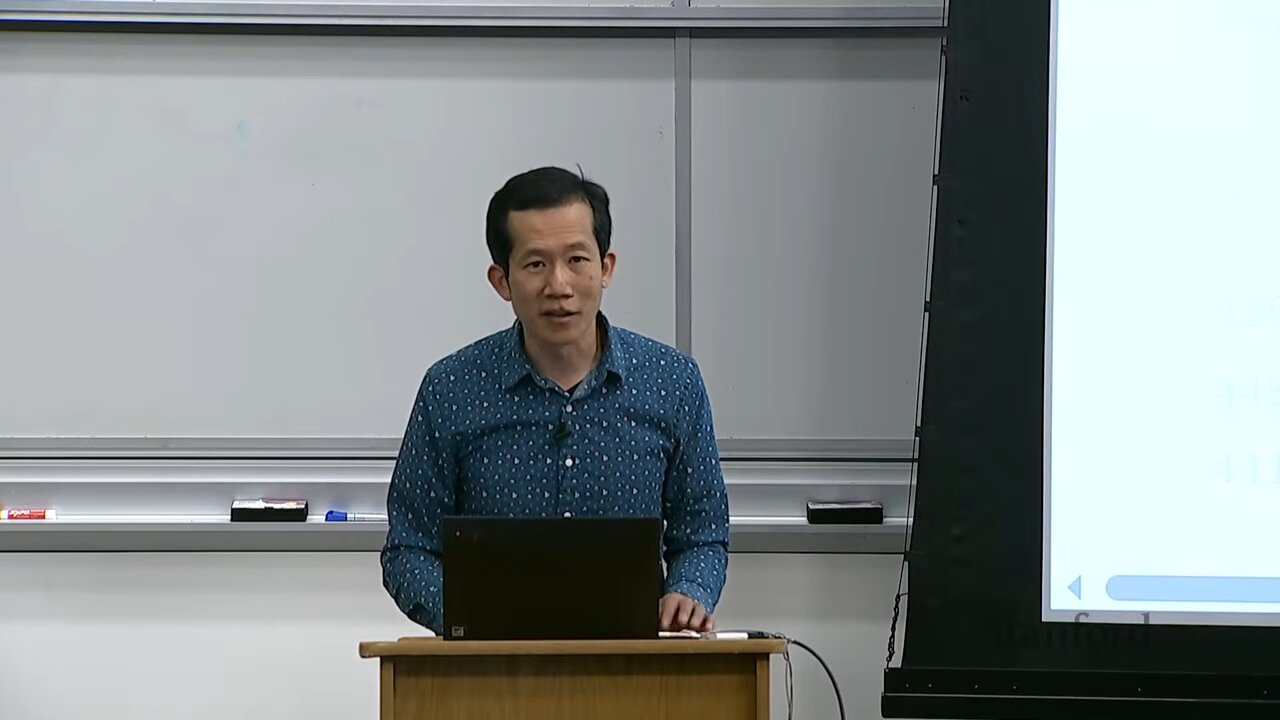
\includegraphics[width=\textwidth]{figures/fig_19_gradient_checkpointing.jpg}
\caption{Gradient checkpointing：只存 $\sqrt{n}$ 个检查点，反向时重算，内存从 $O(n)$ 降到 $O(\sqrt{n})$\protect\footnotemark}
\end{figure}
\footnotetext{视频画面时间区间：40:45--41:15。}

\textbf{Gradient checkpointing}（梯度检查点，又称 activation checkpointing 或 recomputation）是解决激活内存爆炸的关键技术。朴素训练要存所有层的激活（$O(n)$，$n$ 为层数）。checkpointing 的思路：前向时只存\textbf{少数几个}检查点层的输入，其余激活丢弃；反向传播到某层时，从最近的检查点重新做一次前向算出需要的激活。

\begin{importantbox}{以计算换内存}
\[
\text{baseline}: \text{memory} = O(n), \text{compute} = 1\times \text{fwd}
\]
\[
\text{checkpointing}: \text{memory} = O(\sqrt{n}), \text{compute} \approx 1.5\times \text{fwd}
\]
\begin{itemize}
\item 内存从层数线性 $O(n)$ 降到约 $O(\sqrt{n})$（最优检查点策略下）
\item 代价是多算约一次前向（额外 $\sim 33\%$ 计算），即"用计算换内存"
\item 在内存受限（如长序列、大 batch）时极其有用，是训练超大模型的标配
\end{itemize}
\end{importantbox}

\subsection{Checkpointing（模型保存）}

\begin{warningbox}{两种 checkpointing 别混淆}
\begin{itemize}
\item \textbf{Gradient checkpointing}（上节）：训练时省内存的技术
\item \textbf{Model checkpointing}（本节）：把训练状态存盘以防崩溃
\end{itemize}
\end{warningbox}

训练语言模型耗时极长，\textbf{一定会崩溃}。为不丢失进度，需周期性地把状态存盘。要存的不仅仅是模型权重，还包括：
\begin{itemize}
\item \textbf{模型权重}（\texttt{model.state\_dict()}）
\item \textbf{优化器状态}（\texttt{optimizer.state\_dict()}）——否则恢复后 momentum/Adam 状态丢失，训练会抖动
\item \textbf{当前迭代步数}、学习率调度器状态等
\end{itemize}

恢复时把三者都 load 回来，从断点继续。这是工业级训练的基本功。

\subsection{混合精度的实践建议}

\begin{practicebox}{精度选择的工程经验}
\begin{itemize}
\item 默认用 FP32 跑通流程
\item 尽可能切到 BF16（甚至 FP8）做前向，FP32 留给参数更新
\item PyTorch 提供 \texttt{torch.cuda.amp} / autocast 自动管理精度切换，免去手动指定每层的 dtype
\item 前沿方向：FP8 全程训练（数值很挑，需要 trick），甚至 INT4；推理时可以做更激进的 quantization（量化），因为训练比推理对精度敏感得多
\end{itemize}
\end{practicebox}

\begin{knowledgebox}{系统与模型协同设计}
低精度训练的不稳定，部分要靠\textbf{模型架构}来缓解（如更稳的初始化、归一化）。反过来，Nvidia 芯片对低精度（INT4/FP8）有专门加速，这反过来驱动模型设计去适配硬件。这正是第一讲说的"协同设计数据、系统、模型"——Transformer 本身就是 GPU 友好性的产物，未来的架构演进会继续被硬件塑造。
\end{knowledgebox}

\section{总结}

\subsection{核心要点}

\begin{importantbox}{本讲四大要点}
\begin{enumerate}
\item \textbf{资源核算是心态}：要高效，必须精确知道每份 FLOPs 和每字节内存去了哪里——它们直接换算成美元。Napkin math 让你在动代码前就能判断可行性。
\item \textbf{训练 FLOPs $\approx 6ND$}：前向 2 + 反向 4。这个 6 来自链式法则——反向传播每个 matmul 权重要算两个梯度（对 $W$ 和对 $H$），所以反向是前向的两倍。
\item \textbf{内存四件套}：参数 + 梯度 + 优化器状态 + 激活。前三项正比于参数量（AdamW 下约 16 字节/参数），激活正比于 $B \cdot S \cdot d \cdot L$。激活随层数线性增长是深层模型的内存瓶颈。
\item \textbf{BF16 + 混合精度是训练默认}：动态范围（exponent）比精度（fraction）更重要。Gradient checkpointing 用 $\sim 33\%$ 额外计算把激活内存从 $O(n)$ 降到 $O(\sqrt{n})$。
\end{enumerate}
\end{importantbox}

\subsection{与 Assignment 1 的衔接}

本讲用最简单的线性模型讲清了 resource accounting 的\textbf{形式}。Assignment 1 会让你对真正的 Transformer 做同样的分解——矩阵更多、有 attention，但骨架完全一样：参数、激活、梯度、优化器状态四类内存；$6ND$ 的 FLOPs。Percy 强调，亲手在 Transformer 上算一遍，这些概念才会真正扎实。

\subsection{下节预告}

下一讲 Tatsu 会从概念层面讲解 Transformer 架构。届时你将带着本讲建立的"每个 matmul 多少 FLOPs、每层多少激活"的核算直觉，去理解为什么 Transformer 这么设计、哪些变体在什么 scale 下有意义。

\subsection{配套阅读}

\begin{tabular}{p{7cm}p{6cm}}
\toprule
\textbf{材料} & \textbf{对应知识点} \\
\midrule
PyTorch 官方 autograd 教程 & autograd、计算图 \\
Mixed Precision Training (Micikevicius 2017) & 混合精度训练 \\
Adam (Kingma 2014) & Adam 优化器 \\
Decoupled Weight Decay / AdamW (Loshchilov 2017) & AdamW \\
Training Deep Nets with Sublinear Memory (Chen 2016) & Gradient checkpointing \\
H100 / A100 spec sheet & 峰值 FLOPs、tensor core \\
\bottomrule
\end{tabular}

%% --- 正文内容结束 ---

\end{document}
